\documentclass[
english,
ruledheaders=section,%Ebene bis zu der die Überschriften mit Linien abgetrennt werden, vgl. DEMO-TUDaPub
class=report,% Basisdokumentenklasse. Wählt die Korrespondierende KOMA-Script Klasse
thesis={type=Report},% Dokumententyp Thesis, für Dissertationen siehe die Demo-Datei DEMO-TUDaPhd
accentcolor=9c,% Auswahl der Akzentfarbe
custommargins=true,% Ränder werden mithilfe von typearea automatisch berechnet
marginpar=false,% Kopfzeile und Fußzeile erstrecken sich nicht über die Randnotizspalte
%BCOR=5mm,%Bindekorrektur, falls notwendig
parskip=half-,%Absatzkennzeichnung durch Abstand vgl. KOMA-Script
fontsize=11pt,%Basisschriftgröße laut Corporate Design ist mit 9pt häufig zu klein
logofile={img/tuda_logo.pdf}, %Falls die Logo Dateien nicht vorliegen
]{tudapub}


% Der folgende Block ist nur bei pdfTeX auf Versionen vor April 2018 notwendig
\usepackage{iftex}
\ifPDFTeX
\usepackage[utf8]{inputenc}%kompatibilität mit TeX Versionen vor April 2018
\fi


%%%%%%%%%%%%%%%%%%%
%Sprachanpassung & Verbesserte Trennregeln
%%%%%%%%%%%%%%%%%%%
\usepackage[ngerman, main=english]{babel}
% \usepackage[english, main=ngerman]{babel}
% % 中文支持
% \usepackage{fontspec}
% \usepackage{xeCJK}  % LuaLaTeX 也适用

% % 设置中文字体
% \setCJKmainfont{Noto Serif CJK SC}  % 适用于简体中文
% \setCJKsansfont{Noto Sans CJK SC}   % 无衬线字体
% \setCJKmonofont{Noto Sans Mono CJK SC} % 等宽字体

% \usepackage[autostyle]{csquotes}% Anführungszeichen vereinfacht

% Falls mit pdflatex kompiliert wird, wird microtype automatisch geladen, in diesem Fall muss diese Zeile entfernt werden, und falls weiter Optionen hinzugefügt werden sollen, muss dies über
% \PassOptionsToPackage{Optionen}{microtype}
% vor \documentclass hinzugefügt werden.
\usepackage{microtype}
\usepackage{subcaption}
%%%%%%%%%%%%%%%%%%%
%Literaturverzeichnis
%%%%%%%%%%%%%%%%%%%
\usepackage{biblatex}   % Literaturverzeichnis
\bibliography{bibliography}


%%%%%%%%%%%%%%%%%%%
%Paketvorschläge Tabellen
%%%%%%%%%%%%%%%%%%%
%\usepackage{array}     % Basispaket für Tabellenkonfiguration, wird von den folgenden automatisch geladen
\usepackage{tabularx}   % Tabellen, die sich automatisch der Breite anpassen
%\usepackage{longtable} % Mehrseitige Tabellen
%\usepackage{xltabular} % Mehrseitige Tabellen mit anpassbarer Breite
\usepackage{booktabs}   % Verbesserte Möglichkeiten für Tabellenlayout über horizontale Linien
\usepackage{graphicx}
\usepackage{pdfpages}
\usepackage{enumitem}
\usepackage{xcolor}

\usepackage{float}
\usepackage[acronym]{glossaries}
\usepackage{caption}
\captionsetup{justification=centering}
% acronyms
\usepackage{acronym}

%其他引用库
\usepackage{hyperref}



%%%%%%%%%%%%%%%%%%%
%Paketvorschläge Mathematik
%%%%%%%%%%%%%%%%%%%
%\usepackage{mathtools} % erweiterte Fassung von amsmath
%\usepackage{amssymb}   % erweiterter Zeichensatz
%\usepackage{siunitx}   % Einheiten

%Formatierungen für Beispiele in diesem Dokument. Im Allgemeinen nicht notwendig!
\let\file\texttt
\let\code\texttt
\let\tbs\textbackslash
\let\pck\textsf
\let\cls\textsf

\usepackage{pifont}% Zapf-Dingbats Symbole
\newcommand*{\FeatureTrue}{\ding{52}}
\newcommand*{\FeatureFalse}{\ding{56}}

\begin{document}

    \Metadata{
        title=ADP - Charging Station Upgrade to OCPP Communication for Smart Charging,
        author=Junfan Jin, Can Zeng, Yunan Jiang and Huang Chen
    }

    \title{ADP - Charging Station Upgrade to OCPP Communication for Smart Charging}
    \subtitle{}
    \author[J. Jin \and C. Zeng \and Y. Jiang \and H. Chen]{Junfan Jin \and Can Zeng \and Yunan Jiang \and Huang Chen}%optionales Argument ist die Signatur,
    \birthplace{}%Geburtsort, bei Dissertationen zwingend notwendig
    \reviewer{Prof. Dr. Stephan Rinderknecht \and M.Sc Thomas Franzelin \and Dr.Ing. Benjamin Blat-Belmonte}%Gutachter

    %Diese Felder werden untereinander auf der Titelseite platziert.
    %\department ist eine notwendige Angabe, siehe auch dem Abschnitt `Abweichung von den Vorgaben für die Titelseite'
    \department{mb} % Das Kürzel wird automatisch ersetzt und als Studienfach gewählt, siehe Liste der Kürzel im Dokument.
    \institute{IMS}
    \group{}

    \submissiondate{\today}
    \examdate{\today}

    % Hinweis zur Lizenz:
    % TUDa-CI verwendet momentan die Lizenz CC BY-NC-ND 2.0 DE als Voreinstellung.
    % Die TU Darmstadt hat jedoch die Empfehlung von dieser auf die liberalere
    % CC BY 4.0 geändert. Diese erlaubt eine Verwendung bearbeiteter Versionen und
    % die kommerzielle Nutzung.
    % TUDa-CI wird im nächsten größeren Release ebenfalls diese Anpassung vornehmen.
    % Aus diesem Grund wird empfohlen die Lizenz manuell auszuwählen.
    %\tuprints{urn=XXXXX,printid=XXXX,year=2022,license=cc-by-4.0}
    % To see further information on the license option in English, remove the license= key and pay attention to the warning & help message.

    % \dedication{Für alle, die \TeX{} nutzen.}

    \maketitle
    \includepdf[pages=-]{Aufgabenstellung_ADP.pdf}

    % \affidavit % oder \affidavit[digital] falls eine rein digitale Abgabe vorgesehen ist.


    % Es gibt mit Version 3.20 die Möglichkeit ein Bild als Signatur einzubinden.
    % TUDa-CI kann nicht garantieren, dass dies zulässig ist oder eine eigenhändige Unterschrift ersetzt.
    % Dies ist durch Studierende vor der Verwendung abzuklären.
    % Die Verwendung funktioniert so:
    %\affidavit[signature-image={\includegraphics[width=\width,height=1cm]{example-image}}, <hier können andere Optionen wie z.B. affidavit=digital zusätzlich stehen>]

    \tableofcontents

    \clearpage
    \textbf{Abbreviations}
    \begin{acronym}[MPC] % Give the longest label here so that the list is nicely aligned
%\acro{}{}  %sort alphabaticly
\acro{CP}{Charging Point}
\acro{OCPP}{Open Charge Point Protocol}
\acro{EV}{Electric Vehicle}
\acro{V2G}{Vehicle-to-Grid}
\acro{SoC}{State of Charge}
\acro{TX}{transmission}
\acro{RX}{Reciever}
\acro{PP}{Proximity pilot}
\acro{rel}{relay output}
\acro{CSMS}{Charging Station Management System}
\end{acronym}
    \listoffigures
    \listoftables


    % chapter 1
    \chapter{Introduction}

    % section 1.1
    \section{Background}
    With the development of electric vehicles, the demand for charging has also significantly increased, and charging stations can be seen everywhere. However, some charging stations still require users to manually configure settings to use it. Therefore, this ADP aims to optimize and make the charging process intelligent. Users can get a better charging experience without too many setting inputs.
    % section 1.2
    \section{Research Significance}

    The majority of charging stations do not use a unified communication protocol to standardize the charging process, which leads to compatibility issues when vehicles charge at different stations. Many manufacturers use self closed-source charging protocols, such as the Tesla Supercharger Protocol. The reliance on closed-source charging protocols significantly hampers compatibility. Therefore, in this project, the Open Charge Point Protocol (OCPP), an open-source charging protocol, is utilized. For other engineers who may wish to upgrade or modify the system based on this project it is a huge advantage. However, it is evident for code in Python, the OCPP library does not implement certain functionalities. This project aims to optimize the code to address these shortcomings. Moreover, the OCPP protocol is continuously updated, e.g., from version 1.6 to 2.0.1. Each update can alter the library's content; for instance, the JSON files in OCPP 2.0.1 contain much more nested information compared to those in OCPP 1.6. Consequently, it is essential to optimize and upgrade charging stations based on the latest OCPP version to ensure improved functionality and compatibility.

    % section 1.3
    \section{Objectives}

    This project aims to enhance the intelligence of charging stations. The objectives are divided into two parts: software and hardware.

    On the software side, the focus is on enabling communication based on various protocols, such as OCPP, WebSocket, and Modbus, ensuring that different systems can successfully exchange requests and responses to control the charging current.

    Hardware selection is based on the software functionalities. The ultimate goal is to achieve peak shaving, allowing charging stations to charge vehicles with low power during peak electricity demand periods, thereby reducing the burden on the power grid and preventing overload.

    % section 1.4
    \section{Overview}

    The internal structure of the charging station is mainly divided into two parts. The first part is the high-voltage part, which includes components such as the power supply, contactor, fault current protection, and Shelly. This part is responsible for supplying current, monitoring power, and limiting the current to protect users. The second part is the low-voltage section, which handles the charging logic. It consists of a Raspberry Pi, relays, and a level shifter. Additionally, a DC motor controls the locking mechanism of the charging cable. All components are mounted on a DIN rail.

    For the logic control part, the Raspberry Pi offers two charging options. The first option allows users to start charging directly by pressing the start button on the charging station, supplying an AC current of 16A. Charging continues until the stop button is manually pressed. The second option involves using Socket.io to input vehicle information into the Raspberry Pi, including total charging amount, departure time, maximum/minimum current, maximum voltage, and charging mode. The Raspberry Pi then sends an OCPP-format charging needs request message to the optimize system via WebSocket. After optimization, the optimize system returns a set charging profile request message containing the charging schedule. Once the Raspberry Pi receives the charging schedule and confirms that Shelly and EVSE are ready, it initiates the charging process. The optimize system mainly implements a peak-shaving function. During charging, Shelly monitors the charging current and voltage. The Raspberry Pi periodically sends updated charging demand data to the optimize system to refresh the charging schedule.


    % % section 1.5
    % \section{Structure}

    \newpage

    % chapter 2
    \chapter{Hardware Introduction}

    % section 2.1
    \section{EVSE and AF30-30-00-13}

    In order to adjust the current output, the hardware EVSE must be used to adapt the high power input from the supply network to users side. In this case, EVSE WB is used which connects to the level shifter from 3.3 V to 5 V obtaining the communication signals with RX and TX. RX and TX are directly controlled by Raspberry Pi. The EVSE WB consumes power fewer than 1 W while letting default current setting 32 A through which meets our needs.\cite{EVSEdatasheet}

    Meanwhile, EVSE WB is equipped with PP function. It detects the abnormal current passing through cable. \cite{typ2connector} However, for an additional protection from Leakage current, AF30-30-00-13 is connected to rel on EVSE 4-pin side. The maximal working current of AF30-30-00-13 reaches 40 A.\cite{AF30-30-00-13}

    \begin{figure}[htbp]
        \centering
        \includegraphics[width=0.3\textwidth]{img/AF30-30-00-13.jpg}
        \caption{AF30-30-00-13
            (Source: \cite{AF30-30-00-13})}
        \label{fig:AF30-30-00-13}
    \end{figure}


    %插入下 EVSE 的图 (最好自己拍一个?)



    % section 2.2
    \section{Shelly}


    On the load side, it's necessary to monitor the output. Shelly Pro 3 EM captures current, voltage and power by means of flux variation and can be connected with WiFi to transmit the data. The low power consumption under 3 W can also be ignored.\cite{Shelly} As shown in the figure (\autoref{fig:Shelly Pro 3EM}), Shelly Pro 3 EM can be assembled on DIN rail.


    \begin{figure}[htbp]
        \centering
        \includegraphics[width=0.4\textwidth]{img/Shelly Pro 3EM.jpg} % 这里替换成你的图片文件名
        \caption{Shelly Pro 3EM
            (Source: \cite{Shelly})}
        \label{fig:Shelly Pro 3EM}
    \end{figure}



    % section 2.3
    \section{Raspberry Pi 3 Model B+}
    \label{sec:RaspberryIntroduction}

    Raspberry Pi 3B is one of the most important hardware in this case. It has mainly 2 tasks. The first task is to communicate with EVSE through RX and TX to control output voltage. Besides that, Raspberry Pi gives signal to relays in order to drive the locking motor. The overview and the pin-out of Raspberry Pi 3b (\autoref{fig:Raspberry Pi overview}) are shown below.

    \begin{figure}[H]
        \centering
        \includegraphics[width=0.7\textwidth]{img/RaspberryPi3b_and_pin-out.jpg}
        \caption{Raspberry Pi 3b and its pin-out overview
            (Source: \cite{RaspberryPiOverview})}
        \label{fig:Raspberry Pi overview}
    \end{figure}

    %得补充引脚?
    %图片插入的位置不对,后期再调整



    % section 2.4
    \section{Power Supply (3.3V 5V 12V)}

    In this system, different hardware require totally four kinds of voltage supply. The 220 V network serve as the power source from which voltage levels such as 3.3 V, 5 V and 12 V are adapted.

    Firstly, Phoenix STEP3-PS provides 5 V 3 A current for Raspberry Pi on the input side. Then, Raspberry Pi outputs also 5 V voltage not only as Vcc for relay but also for level shifter on the high voltage side. Secondly, Mean Well NDR75-12 transforms 220 V into 12 V 6.3 A current which supplys the relay. Meanwhile, Raspberry Pi outputs signals with 3.3 V on GPIO14 and GPIO15, this will be converted by level shifter into 5 V signals to EVSE. The electrical connection is demonstrated by circuit diagram in appendix.

    % section 2.5
    \section{Connector (Typ 2)}

    %这里带过介绍下其他的connectors

    There are various connector standards, such as SAE J1772(\autoref{fig:SAEJ1772}), which is implemented in North America but only supports single-phase AC. Another example is Tesla's SAE J3400(\autoref{fig:SAEJ3400}), which supports both single-phase AC and DC charging.

    \begin{figure}[htbp]
        \centering
        \begin{subfigure}[b]{0.4\textwidth}       \includegraphics[width=\textwidth]{img/SAEJ1772.jpg}
            \caption{SAE J1772}
            \label{fig:SAEJ1772}
        \end{subfigure}
        \hfill
        \begin{subfigure}[b]{0.4\textwidth}
            \includegraphics[width=\textwidth]{img/SAEJ3400.jpg}
            \caption{SAE J3400}
            \label{fig:SAEJ3400}
        \end{subfigure}
        \caption{pin-out for both standards(Source: \cite{SAEJ1772} and \cite{SAEJ3400})}
        \label{fig:2standardpinout}
    \end{figure}



    In this project, a IEC 62196-2 connector (Type 2) is used, which has seven pins. L1, L2, and L3 correspond to the three-phase power lines, while N represents the neutral line. PP and CP are signal lines for pre- and post-insertion signalling, respectively. PE is the ground wire.

    \begin{figure}[H]
        \centering
        \includegraphics[width=0.4\textwidth]{img/pin-out_for_typ2.jpg} % 这里替换成你的图片文件名
        \caption{pin-out for typ2 connector
            (Source: \cite{typ2connector})}
        \label{fig:typ2pin-out}
    \end{figure}


    % section 2.6
    \section{Motor and relay}

    Connection between CP and charging cable can be flexibly established or removed. To prevent accidental unplugging of the charging cable during charging, which could lead to electric shock incidents, a motor is installed at the interface of the charging station to lock the cable in place during charging, making it impossible to unplug the cable. The motor's forward and reverse rotation is controlled by a dual-channel relay.

    % 继电器的电路导通细节应该简单的介绍吗?

    \newpage
    % chapter 3
    \chapter{Software Introduction}

    % section 3.1
    \section{OCPP}
    \label{sec:ocppIntroduction}

    OCPP is a protocol developed and maintained by the Open Charge Alliance (OCA). In terms of device management, charging stations can send detailed diagnostic data to the CSMS, facilitating maintenance. It also utilizes ISO 15118 for secure vehicle authentication. \cite{OCPP}The primary reasons for using OCPP in this project are its good compatibility and existing libraries in python.

    At the start of this project, Version 2.0.1 was the latest version of the protocol. Compared to OCPP 1.6, OCPP 2.0.1 offers more detailed message definitions in the JSON files, enhanced security features, and greater compatibility. And the official OCPP library already exists in Python.\cite{ocpplibrary} Though the latest official version is v2.0.0, but before the start of this project, the latest version was v1.0.0, that's why this project uses v1.0.0. Due to significant changes in the latest official library, it no longer supports the old version's enumeration classes. Therefore, the library used in this project is not compatible with the latest version.


    % section 3.2
    \section{WebSocket}
    \label{sec:websocketIntroduction}

    % (咱们项目中,树莓派既是客户端又是服务端 ! ) 这一块补充说明optimize system和client?
    Thanks to full-duplex communication, \texttt{WebSocket} allow the client and server to send and receive data simultaneously without waiting for a response from the other side. In this project, Raspberry Pi is not only server but also client. Unlike HTTP’s request-response model, once a \texttt{WebSocket} connection is established, data can be transmitted at any time, reducing communication delay.\cite{websockets}  The \texttt{WebSocket} connection remains open until either the client or server actively closes it.

    However, instead of manually opening and closing the connection, the context manager is used in this project to automatically manage the connection. The details will be explained in section 4.2. Although Socket is available, the official libraries use asychronous \texttt{WebSocket} communication. Due to consistency this project follows that.


    % section 3.3
    \section{Modbus}
    \label{sec:modbusIntroduction}

    The Raspberry Pi communicates with the EVSE via Modbus . Modbus adopts a Master-Slave architecture and supports multiple communication methods, including Modbus RTU, Modbus ASCII, and Modbus TCP.\cite{modbus}

    Modbus uses serial communication, which transmits data bit-by-bit through one or multiple data cables.Typical baud rates are 9600/19200/115200 bps.almost all industrial devices, such as PLCs, HMIs, and EVSEs, support Modbus.Additionally, using RS-485, can communicate with up to 247 devices. If in further case, there is a demand for communication with multiple CPs, it's also extendable.


    % section 3.4
    \section{Coroutine and Thread}
    \label{sec:CoroutineThreadIntroduction}

    A process can have multiple threads, and threads are used to execute multiple concurrent (assumed that CPU has one core) or parallel (assumed that CPU has multiple core) operations within a single program. Different to threads, coroutines are program that allow execution to be suspended and resumed. While excuting different tasks coroutines don't need to switch the context or with low switching-context cost. Context refers to the execution state of a program at a given moment, including register information, the call stack, memory data and so on. When the CPU switches between different tasks (threads, processes, or coroutines), it needs to save the current task's state and restore the next task's state to ensure continuous execution.\cite{coroutinewiki}

    \begin{table}[htbp]
        \centering
        \label{tab:threadandcoroutine}
        \begin{tabular}{|l|c|c|}
            \hline
            \textbf{Characteristic} & \textbf{Multi-Thread} & \textbf{Coroutine}\\
            \hline
            Blocking                & Yes & No\\
            \hline
            Switching context cost  & High & Low\\
            \hline
            Memory usage            & High & Low\\
            \hline
            Execution Modes         & Concurrency / Parallelism & Concurrency\\
            \hline
            Execution Layer         & Kernel Mode & User Mode\\
            \hline
            Scheduler               & Operating System Scheduler & Self-Scheduling by Programs\\
            \hline
        \end{tabular}
        \caption{Comparison between Thread and Coroutine}
    \end{table}


    Frequent I/O operations means that during execution, a program frequently reads or writes data rather than continuously calculating. In the case of vehicle charging, the computational demand of charging stations is not high; instead, they require frequent command reading.From the table, we can see that coroutines are non-blocking, this prevents situations where the CPU is occupied but not actively utilized during frequent I/O operations. \cite{threadcoroutine}Therefore, in such scenarios, coroutines are more suitable than threads.

    %这里如果要进一步说明thread在执行顺序上的区别 可以加入thread coroutine的时序图并且语言简单描述下 ?

    It is important to note that if a function calls await inside, it must be declared as async because await can only be used within a coroutine function. The higher-level function that calls this async function must also use await to wait for its result, which means the higher-level function must also become async. In other words, async and await always appear in pairs, and they can force functions that initially do not require asynchronous operations to be modified into asynchronous functions as well.

    % section 3.5
    \section{Signal and Slot}
    \label{sec:signalSlotIntroduction}

    The Signal and Slot was first introduced in the Qt framework to reduce coupling between different system modules. It allows components to interact without depending on each other. A single signal can be connected to multiple slot functions while a single slot function can also be connected to multiple signals, making the system more flexible.

    Because this construct is event-driven, it is well-suited for handling events and executing the corresponding code logic. Compared to callback functions, signals allow dynamic connections and disconnections of slot functions, whereas callbacks must be defined beforehand. Thus, the modification of the call of callback functions during execution is impossible. However, signals connect to slot functions dynamically, it can be challenging to explicitly check signal connections, especially when the definitions of signal connections are distributed across different classes or modules. Thus, tracking calls of functions and methods becomes very difficult during the occurrence of bugs.

    % % section 3.6
    % \section{front-end and back-end}
    % \label{sec:frontEndIntroduction}

    % In order to remote system operation and transmit data during usage, it need to develop a front-end interface. In this project, it is enough to build the web frontend, meanwhile,  a \texttt{WebSocket} interface is reserved for further development

    % The web front end is primarily implemented using HTML, CSS, and JavaScript, supporting basic data interaction, inspection, and visualization. HTML is mainly used for structuring the web page, CSS for styling, and JavaScript for handling user interactions and dynamically updating the page content.

    % There are various ways to implement the web back end, such as Django, Flask, Qt, and Pyramid etc. Since this project has relatively few requirements and does not demand high concurrency, chosing Flask to build a lightweight web server is optimal.


    % chapter 4
    \chapter{System Base}
    \label{chap:SystemBase}

    % This chapter mainly introduces the design of the software's framework for the project which is used between the optimizer and the Raspberry Pi charging station. It includes the following aspects:

    % \begin{enumerate}
        %     \item The Frame of Systems
        %     \item The design of WebSocket communication ports.
        %     \item Methods for obtaining and generating OCPP data
        %     \item The adaptation of the official library
        %     \item The design of the signal-slot construct
        %     \item Application and isolation of synchronous and asynchronous programming
        % \end{enumerate}


    %本章主要是介绍该项目系统框架的软件底层部分的设计,其在优化器与树莓派充电桩部分中共同使用,包括系统框架简介,\texttt{WebSocket}通讯端口设计,获取OCPP数据的方式,生成OCPP数据的方式,对于官方库机制的使用以适配,信号槽机制的设计,同步与异步编程的使用与隔离
    \section{System Frame}
    \label{sec:SystemFrame}

    \begin{figure}
        \centering
        \includegraphics[width=1\textwidth]{img/SimpleClassDiagram.png}
        \caption{System Frame}
        \label{fig:SystemFrame}
    \end{figure}
    % 本项目主要包含两个核心系统:充电桩系统和优化器系统,二者的功能和结构相似,如上图所示。优化器系统由两个主要模块构成:通讯层和服务层。通讯层负责接收各类消息并进行解析,能够处理OCPP(开放充电桩协议)消息、图片、文本消息等格式,此外还需要管理和维护与网页服务器的通信,确保数据流畅传递至客户端界面。服务层则是优化器系统的核心,主要负责处理具体的优化器业务逻辑,包括计算充电计划表、负载均衡以及数据分析等功能。

    % 充电桩系统除了包含优化器系统的通讯层和服务层外,还增加了一个硬件层,这一层的主要职责是管理硬件设备(如充电桩硬件、传感器等)并与硬件进行通讯。硬件层与系统其他部分的集成非常重要,它确保硬件设备能够正常工作并实时反馈状态。硬件层的数据处理还涉及到对充电桩的开关控制、计划表执行、故障检测等多项功能。

    % 在充电桩系统的通讯层,除了基本的消息接收和解析功能外,还特意增加了WebSocket端口功能。这个WebSocket端口是为了支持与未来可能开发的新设备进行通讯。这一设计为系统的扩展性提供了便利,使得在今后新设备或功能的加入时,不会受到当前通讯方式的限制。

    % 此外,两个系统间通过WebSocket端口进行通信

    This project primarily consists of two core systems: the charging point system and the optimizer system. The functionalities and structures of these two systems are similar, as illustrated in the diagram above.

    The Optimizer System is composed of two main modules: the Communication Layer and the Service Layer. The Communication Layer is responsible for receiving and parsing various types of messages, including OCPP (Open Charge Point Protocol) messages, images, and text messages. Additionally, it manages and maintains communication with the web server to ensure smooth data transmission to the client interface. The Service Layer, which is the core of the Optimizer System, handles the primary business logic, such as calculating charging schedules, load balancing, and data analysis.

    The Charging Point System, in addition to the Communication Layer and Service Layer found in the Optimizer System, incorporates an additional Hardware Layer. The primary role of this layer is to manage hardware devices (such as charging point hardware and sensors) and facilitate communication with them. The integration of the Hardware Layer with other system components is crucial, ensuring that hardware devices function properly and provide real-time feedback. This layer also handles key operations such as switching the charging point on and off, executing charging schedules, and detecting faults.

    In the Communication Layer of the Charging point System, besides basic message reception and parsing capabilities, a \texttt{WebSocket} port has been specifically added. This \texttt{WebSocket} port is designed to support communication with new devices that may be developed in the future. This design enhances the system's scalability, ensuring that future additions of new devices or functionalities will not be restricted by the current communication method.

    Additionally, the communication between the two systems is also realized via \texttt{WebSocket} port.


    \section{WebSocket ContextManager}
    \label{sec:websocketContextManager}

    To enhance the expansibility and flexibility of the system, this project fully considers the potential need for dynamic opening or closing of \texttt{WebSocket} ports. Especially in real application, \texttt{WebSocket} ports may need to be reconnected, closed, or switched at any time due to various demands or changes in the network environment, for instance, CP must get "Authorize" before charging, but while charging the system accesses "MeterValue". those demands are not taking place at the same time. To make managing the lifecycle of \texttt{WebSocket} ports more convenient and robust, the project introduces a context manager construct to handle the entry and exit of \texttt{WebSocket} connections in general.


    %为了提升系统的扩展性和灵活性,本项目设计时充分考虑到\texttt{WebSocket}端口可能存在动态开放或关闭的需求。尤其在实际应用场景中,\texttt{WebSocket} 端口可能因不同业务需求或网络环境的变化而随时进行重连、关闭或切换。为了能够更加方便且安全地管理 \texttt{WebSocket} 端口的生命周期,项目引入了 上下文管理器机制,用于统一管理 \texttt{WebSocket} 连接的进入和退出过程。


    %By using a context manager, the process of opening and closing \texttt{WebSocket} ports is encapsulated within the \_\_enter\_\_ and \_\_exit\_\_  methods. Developers can simply use a with statement to ensure that the connection is automatically established when entering the context and properly closed with resources released when exiting. And  for the asynchronous case, \_\_aenter\_\_ and \_\_aexit\_\_ are used. This design not only simplifies the \texttt{WebSocket} port management process and prevents issues like forgetting to close connections or resource leaks in case of unexpected exits but also reduces the need for try/finally statements, improving code readability and maintainability.


    %通过使用上下文管理器,\texttt{WebSocket} 端口的打开与关闭过程被封装在 \_\_enter\_\_ 和 \_\_exit\_\_ 方法中,开发者只需使用 with 语句即可确保在进入上下文时自动建立连接,在退出时自动关闭连接并释放资源。(补充:在异步的例子中使用 \_\_aenter\_\_ 和 \_\_aexit\_\_ )这样设计不仅简化了 \texttt{WebSocket} 端口的管理流程,避免了忘记关闭连接或异常退出时资源泄漏的问题,还减少使用try/finally这些语法,增强了代码的可读性和可维护性。


    By applying the context manager, the opening and closing process of the \texttt{WebSocket} port is encapsulated in the \texttt{\_\_enter\_\_} and \texttt{\_\_exit\_\_} methods. Developers simply use the \texttt{with} statement; the connection is automatically established upon entering the context and closed upon exiting. And for the asynchronous case, \texttt{\_\_aenter\_\_} and \texttt{\_\_aexit\_\_} are used. And the resources are also released. This design not only simplifies the management process of the \texttt{WebSocket} port, avoids the problem of resource leakage when the connection closure is forgotten or an abnormal exit occurs, but also enhances the readability and maintainability of the code.

    %此外,上下文管理器机制为后续功能扩展提供了良好的基础。例如,未来若需在连接建立或断开时增加日志记录、异常捕获或权限校验等操作,只需在上下文管理器中扩展相应逻辑即可,无需改动主业务流程代码,极大地提高了系统的可扩展性和安全性。

    In addition, the context manager provides a good foundation for subsequent function expansion. For example, if logging, exception handling, or permission verification needs to be added during connection establishment or disconnection, this can simply be achieved by extending the corresponding logic in the context manager without modifying the core logic, which significantly enhances the system's extensibility and security.

    %值得一提的是,目前本项目中 \texttt{WebSocket} 端口实例直接组合在 \texttt{OCPP} 消息端口类中,存在一定的耦合关系。这种设计方式虽然实现简单、便于快速开发,但从软件架构设计的角度来看,\texttt{WebSocket} 层与\texttt{OCPP} 协议层紧密绑定,两者生命周期强相关,不利于后续功能的扩展与维护。

    It is worth mentioning that in this project, the \texttt{WebSocket} port instance is directly integrated in the \texttt{OCPP} message port class, and create a certain coupling. This design is simple to implement and facilitates quick development. However, from a software architecture perspective, the \texttt{WebSocket} layer is closely coupled with the \texttt{OCPP} protocol layer, and the life cycles of the two are strongly related, which hinders the expansion and maintenance of subsequent functions.

    % 个人感觉这里的这里可以提一句:To further decouple the system, some suggestions are offered in \section{Discussion}

    %为了解决这个问题,更优雅的设计方式是:单独抽象(用“分离”这个词个人感觉会好些)出\texttt{WebSocket} 端口管理类,采用单例模式实现全局唯一的管理器。管理器内部维护\texttt{WebSocket} 连接池,按\texttt{id}或连接地址、端口进行管理与复用。\texttt{OCPP} 协议端口类只需通过管理器获取或注册所需的\texttt{WebSocket} 连接即可,彻底解耦\texttt{WebSocket} 层与\texttt{OCPP} 协议解析层,同时提升资源复用率。

    To solve this problem, a more elegant design is to abstract the \texttt{WebSocket} port management into a  class, and use the singleton mode to create the only instance - a globally unique manager.The manager maintains the \texttt{WebSocket} connection pool internally which manages and reuses connection based on connection ID, address and port. The \texttt{OCPP} protocol port class only needs to obtain or register the required \texttt{WebSocket} connection through the manager, fully decoupling the \texttt{WebSocket} layer and the \texttt{OCPP} protocol parsing layer, while improving the resource reuse rate.



    %这里可以放到Disscusion?




    \section{Python Library OCPP}
    \label{sec:ocppLib}
    %在python中已有OCPP的官方库,库中包括4个部分,分别为\texttt{ChargePoint}模块,路由(routing)模块,v1.6与v2.0.1的枚举类、数据类等数据定义,以及报错和信息模块。其使用流程为先通过路由模块注册方法,然后启动\texttt{ChargePoint}模块并通过对\texttt{WebSocket}持续监听获取消息,或手动将\texttt{WebSocket}接收的信息传给\texttt{ChargePoint}。注册方法形参是接收的消息,返回值为发送的响应消息。其中注册方法的方式是通过使用\texttt{ocpp.routing}中定义的装饰器\texttt{@on(ocpp.enum.Action) @after(ocpp.enum.Action)}对被注册的函数进行装饰,装饰器是在对应的\texttt{ocpp.enum.Action}中创建注册方法列表,将被装饰的函数名添加其中,随后在\texttt{CP}实例化时,将函数与之绑定。当接收消息并解析时,将执行注册方法列表中绑定的函数。
    %该方法的优点在于使用方便,无需额外进行注册的设置或声明,条理清晰,在注册方法定义处即得知其与哪个消息动作绑定。但是该官方库的函数注册实现方式限制了该系统不支持高并发操作,不支持多函数注册以及注册方法必须在\texttt{ocpp.charge\_point.ChargePoint}类中定义。其原理如下:

    There exists an official library of OCPP in Python, which includes 4 parts, namely the \texttt{ChargePoint} module, the \texttt{Routing} module, the enumeration class and data class of v1.6 and v2.0.1, and the error and information module. The procedure is to first register the method through the routing module, then start the \texttt{ChargePoint} module and obtain messages by continuously listening to \texttt{WebSocket}, or manually pass the information received by \texttt{WebSocket} to \texttt{ChargePoint}. The formal parameter of this registration method is the received message, and the returned value is the sent response message. The registration method is to decorate the registered function by using the decorators \texttt{@on(ocpp.enum.Action) and @after(ocpp.enum.Action)} defined in \texttt{ocpp.routing}. The decorator creates a registration method list in the corresponding \texttt{ocpp.enum.Action}, adds the decorated function name into it, and then binds the function to it when \texttt{ChargePoint} is instantiated. When the message is received and parsed, the bound function in the registration method list will be executed.
    The advantage of this method is that it is easy to use, requiring no additional registration settings or declarations. It is well-organized, and the message action to which the registration method is bound can be easily identified at the method definition.

    However, the official library's function registration implementation method has several limitations:
    \begin{enumerate}
        \item no support for high-concurrency operations
        \item no support for multi-function registration
        \item all registered methods must be defined within the \texttt{ocpp.charge\_point.\\ChargePoint} class
    \end{enumerate}
    The principle is as follows:
    \begin{itemize}
        \item %代码行%\texttt{ocpp.charge\_point.ChargePoint.\_handle\_call(self, msg), line 284}中获取被\texttt{@on}注册的方法时,使用的是字典的映射来直接绑定的。当调用注册方法处理第一个消息时,如果此时传进第二个相同消息动作的消息,则第二个消息只能等待第一个消息处理完才能被接着处理。这样当存在多客户端发送相同请求时,系统可能会因为无法处理后续消息而导致响应超时。然而由于需要更改ocpp库,考虑到代码可能增加移植在别的设备的难度,项目中我们并未对库进行修改,但我们提出了两个可能的解决方法:

        In line 284 of the code \texttt{ocpp.charge\_point.ChargePoint.\_handle\_call\\(self, msg)}, when the code trying to get the method registered with \texttt{@on}, it applies directly bound using a dictionary mapping. When the first message is being processed by the registered method and a second message with the same action is received, the second message has to wait for the first one to finish processing before it can be handled. As a result, when multiple clients send the same request, the system may experience a response timeout due to its inability to process subsequent messages in time.

        However, modifying the \texttt{OCPP} library could introduce potential errors and increase the difficulty of porting the code to other devices, so we chose not to modify the library. Instead, we propose two possible solutions:

        \begin{itemize}
            \item %对库的注册结构进行更改,不修改传递消息的格式。可以在\texttt{@on}注册方法时,注册一个工厂,当接收到消息后,应该由工厂生产方法,然后执行生产出的方法,而非工厂函数,这样就将消息传入和执行进行了分离解耦,然后将被执行的方法加上时间戳,放入执行队列中,使用另一个对象对队列进行监听。如果超时,则强制中断方法的执行,销毁方法对象并移出队列,同时返回超时的信号,当列表为空时则停止监听。这样通过动态生成、管理执行对象就实现了对同时接收多个同消息动作的消息处理的支持。

            Change the registration structure of the library without modifying the format of the message transmission.
            Register a factory when registering a method in \texttt{@on}. When a message is received, the factory should produce a method and then execute the produced method instead of the factory function. This separates and decouples the message input and execution. Then add a timestamp to the executed method, put it in the execution queue, and use another object to monitor the queue. If a timeout occurs, the execution of the method is forced to be interrupted, the method object is destroyed and removed from the queue, and a timeout signal is returned. When the list is empty, the listening will be stopped. In this way, by dynamically generating and managing execution objects, support for message handling when receiving multiple messages with the same action at the same time is achieved.

            \item %对库的注册结构进行更改,同时修改传递消息的格式。不使用装饰器的方式注册方法,而是使用信号(\ref{sec:signal})对其连接,同第一种方法一样分离处理消息和接收消息的动作,然而需要再请求端发送时同时数据的发送时间戳,然后将执行方法加入队列,启动监听循环,当消息超时,则移出队列,并反馈/报错消息超时。与第一种方法的不同点在于,使用信号可以同时解决不能对一个动作注册多个方法的问题

            Change the registration structure of the library and modify the format of the message transmission. Instead of using decorators to register methods, it is also possible to use signals (\ref{sec:signal}) to connect them. Like the first approach, this separates the actions for handling and receiving messages. However, it requires the sender to send a timestamp with the data. Then add the execution method to the queue and start the listening loop. If a message times out, it is removed from the queue, and a timeout error is returned. The difference from the first method is that using signals can solve the problem of not being able to register multiple methods for one action at the same time.

        \end{itemize}

        \item %代码行\texttt{ocpp.routing.create\_route\_map(obj),line 134}中使用字典定义了注册方法的映射,然而由于使用的是\texttt{routes[action][option] = attr}直接赋值的方式,会导致同时被相同消息动作的装饰器装饰注册时,例如\texttt{@on(Action.authorize)},后被装饰的函数将覆盖之前装饰的函数,因此不支持注册多函数处理同一个消息动作。

        The code line \texttt{ocpp.routing.create\_route\_map(obj), line 134} uses a dictionary to define the mapping of the registration method. However, since the direct assignment method \texttt{routes[action][option] = attr} is used, when a function is registered with the decorator of the same message action at the same time, for example \texttt{@on(Action.authorize)}, the function decorated later will overwrite the function decorated earlier. Therefore, it does not support registering multiple functions to handle the same message action.

        %\item %代码行\texttt{ocpp.routing.create\_route\_map(obj),line 120}中使用了\texttt{attr = getattr(obj, attr\_name)}方法获取注册方法/方法,而在\texttt{ChargePoint}中实例化时,向\texttt{ocpp.routing.create\_route\_map(obj)}传入的参数为self,即\texttt{ChargePoint}本身,所以当注册方法被定义在其他非\texttt{ChargePoint}类及其子类中时,将不会被注册,接收到相关消息动作时将不会调用函数进行处理。因此注册方法定义被严格限制在\texttt{ocpp.charge\_point.ChargePoint}类中。

        \item The code line \texttt{ocpp.routing.create\_route\_map(obj), line 120} uses the \texttt{attr = getattr(obj, attr\_name)} method to obtain the registration method/method, and when instantiated in \texttt{ChargePoint}, the parameter passed to \texttt{ocpp.routing.create\_route\_map(obj)} is \texttt{self} , that is, \texttt{ChargePoint} itself, so when the registration method is defined in other non-\texttt{ChargePoint} classes and their subclasses, it will not be registered, and the function will not be called for processing when receiving related message actions. Therefore, the registration method definition is strictly limited to the \texttt{ocpp.charge\_point.ChargePoint} class.
    \end{itemize}

    \section{Method to get OCPP data}
    \label{sec:ocppSendReceive}
    % \texttt{OCPP}官方库中给出的获取数据方式是通过对方法进行注册,在注册方法的形参中获取消息的一级键名,而这些形参在接受消息时会被自动解包赋值,于是就得到了对一层json数据的展开数据。而发送响应则是在注册方法中返回包含响应数据的指定的数据类。
    % 然而该方法存在接收消息,处理消息,返回消息的耦合,当情况复杂时代码难以扩展。为了对该方法进行解耦,本项目将使用信号\ref{sec:signal}分离接收的消息,OCPP消息信号一共有三种:

    In the \texttt{OCPP} official library, data is obtained by registering a method, where the first-level key name of the message is passed as a parameter to the registration method. These parameters are automatically unpacked and assigned when the message is received, providing the expanded data of one layer of \texttt{JSON}. To send a response, the registration method returns a data class containing the response data.
    However, this method couples the receiving, processing, and returning of messages, making it difficult to extend when the situation becomes more complex. To decouple this process, this project will use signals (see \ref{sec:signal}) to separate the message reception. There are three types of \texttt{OCPP} message signals(\autoref{fig:signalMsgCommunication}):

    \begin{itemize}
        %\item \texttt{signal\_request} 用于接收传递请求方发来的请求信息,信号的具体内容为包含时间戳,消息动作,消息id,以及消息内容的一个字典
        %\item \texttt{signal\_response} 用于接收传递接收方发来的响应信息,信号的具体内容为包含消息动作,请求消息,响应消息,请求消息的时间戳,响应消息有效性的状态(成功收到响应,响应超时,接收错误)的一个字典。当请求发送方发送请求等待响应消息超时的时候,将自动接收到一个含有响应消息有效性状态为响应超时的信号数据。
        % \item \texttt{signal\_response\_result} 用于传递接收方发送响应消息后的结果,信号具体内容为包含消息动作,请求消息的时间戳,响应消息,发送结果(在有效时间内成功发送响应,超时发送,发送错误)的一个字典。由于请求消息发送后一定会有响应消息返回,但是响应消息发送后,系统难以知道是否在规定时间内返回了响应消息。于是基于系统中的自查,将对响应消息的结果进行反馈。此信号可以用于对某些固定数据进行缓存处理,当出现高频的请求时,可以直接使用上一次未成功发送的数据,减少计算时间。然而本项目暂时没有高频请求的需求,故只创建了信号,未使用该信号。

        \item \texttt{signal\_request} is used to receive the request information sent by the requester. The specific content of the signal is a dictionary containing timestamp, message action, message id, and message content. \item \texttt{signal\_response} is used to receive the response information sent by the receiver. The specific content of the signal is a dictionary containing message action, request message, response message, timestamp of request message, and status of response message validity (successful response received, response timeout, reception error). When the request sender times out while sending a request waiting for a response message, a signal data containing the response message validity status of response timeout will be automatically received.
        \item \texttt{signal\_response\_result} is used to transmit the result after the receiver sends a response message. The specific content of the signal is a dictionary containing message action, timestamp of request message, response message, and sending result (successful response sent within the valid time, timeout sending, sending error). After a request message is sent, a response message will be returned. However, after the response message is sent, it is difficult for the system to know whether the response message is returned within the specified time. Therefore, based on the self-check in the system, the result of the response message will be fed back. This signal can be used to cache certain fixed data. When there are high-frequency requests, the data that was not successfully sent last time can be used directly to reduce the calculation time. However, this project does not have the need for high-frequency requests for the time being, so only the signal is created and not used.
    \end{itemize}
    \begin{figure}[H]
        \centering
        \includegraphics[width=1\linewidth]{img/SignalMsgCommuication.png}
        \caption{Message Communication}
        \label{fig:signalMsgCommunication}
    \end{figure}

    % 而发送OCPP数据则是通过手动调用\texttt{send\_response\_message}与\texttt{send\_request\_message}方法发送数据,分离了接收请求消息与发送响应消息的关系。

    % 由于该项目未改变原来ocpp库的代码,所以仍是通过注册获取信息,然而注册方法的返回则是调用一个\texttt{while}循环方法,该方法中循环监听响应消息队列,并检查时间是否超时。当消息队列存在消息时,退出循环并返回消息给注册方法,注册方法返回响应消息,通过\texttt{ChargePoint}类发送响应消息。其中消息队列用于隔离同步与异步程序,同时支持多消息排队等候发送。检查时间可以设置预估网络延迟时间和提前发送时间,例如标准timeout为30s,预估网络延迟为5s,提前发送时间为1s,则实际允许等待的时间为24s,超时则将自动返回默认消息,同时向系统反馈超时发送。

    Since the in the project we do not change the code of the original \texttt{OCPP} library, information is still obtained via registration. However, the return of the registration method is to call a \texttt{while} loop method, which loops to listen the response message queue and checks whether a timed out occurs. When there is a message in the message queue, exit the loop and return the message to the registration method. The registration method returns the response message and sends the response message through the \texttt{ChargePoint} class. The message queue is used to isolate synchronous and asynchronous programs, and supports multiple messages waiting to be sent in queue. The check time can set the estimated network delay time and the advance sending time. For example, the standard timeout is 30s, the estimated network delay is 5s, and the advance sending time is 1s. The actual waiting time allowed is 24s. If the timeout exceeds, the default message will be automatically returned, and the timeout will be fed back to the system.

    \section{Method to generate OCPP data}
    \label{sec:ocppGenerator}
    % 相对于层级结构简单,最大层级仅有两层的ocpp 1.6 的消息格式,ocpp 2.0.1的消息格式在结构上则显著复杂得多,消息的层级更深且不固定,甚至存在4层以上的复杂层级关系。虽然现有的 OCPP 库中提供了相应的消息数据类用于封装消息内容,但在实际编码过程中,开发者仍然需要手动对这些数据类赋值或直接构造复杂的嵌套字典结构。这种手动构建消息的方式存在显著的风险和问题。首先,由于 OCPP 2.0.1 中的数据字段极为丰富,字段之间存在大量的类型约束、必填与选填的限制关系,以及嵌套结构的要求,开发者在手动构建过程中极易因疏忽而填错字段、遗漏关键参数或违反字段约束,进而导致 OCPP 消息在传输过程中被拒绝或通信失败。其次,开发者在面对庞大的协议标准时,往往需要频繁查阅官方 JSON Schema 或文档,以确认字段名称、数据类型及其含义,增加了开发成本,降低了开发效率。为了解决上述问题,降低 OCPP 消息构建过程中的出错概率,并提升开发效率,本项目设计并实现了一种参考于建造者模式思想,且充分发挥IDE的DocString提示功能的ocpp消息生成器用来创建ocpp消息。生成器的核心思想是将 OCPP 消息的复杂结构封装在函数接口中,开发者无需关注底层的嵌套关系和字段约束,仅需按照函数的参数提示逐级调用并完成数据填充即可自动生成符合 OCPP 协议标准的数据类或字典。

    Compared with the message format of \texttt{OCPP 1.6}, which has a simple hierarchical structure and only two layers at the maximum, the message format of \texttt{OCPP 2.0.1} is significantly more complex in structure. The message hierarchy is deeper and not fixed, and sometimes exceeds four layers. Although the existing \texttt{OCPP} library provides corresponding message data classes for encapsulating message content, in the actual coding process, developers still need to manually assign values to these data classes or directly construct complex nested dictionary structures. This manual approach introduces significant risks and challenges. First, due to the extremely rich data fields in \texttt{OCPP 2.0.1}, there are a large number of type constraints, mandatory and optional restrictions between fields, and nested structure requirements. Developers are very likely to fill in the wrong fields, omit key parameters, or violate field constraints due to negligence during the manual construction process, which will cause \texttt{OCPP} messages to be rejected or communication fails during transmission. Secondly, when facing a large number of protocol standards, developers often need to frequently refer to the official \texttt{JSON} Schema or documents to confirm the field name, data type and its meaning, which increases development costs and reduces development efficiency. In order to solve the above problems, reduce the error probability in the process of building \texttt{OCPP} messages, and improve development efficiency, this project designed and implemented an \texttt{OCPP} message generator that refers to the builder pattern and fully utilizes the \texttt{DocString} prompt function of the IDE to create \texttt{OCPP} messages. The core idea of the generator is to encapsulate the complex structure of the \texttt{OCPP} message in the function interface. Developers only need to follow level-by-level prompts to fill in the data, automatically generating a data class or dictionary that conforms to the \texttt{OCPP} protocol standard, without worrying about the underlying nested structures or field constraints.

    % 具体而言,OCPP 消息生成器以函数的形式存在,函数的形参即为单层数据的各个字段名,实参则为对应的字段值。函数内部根据 OCPP 协议的定义自动完成数据的封装和结构构建,最终返回符合标准的数据对象。由于生成器函数配备了完善的类型注解和文档字符串,开发者在使用主流 IDE编写代码时,IDE 能够自动识别函数的参数类型、限制条件及字段描述,直接在代码编辑过程中给予开发者完整的提示和校验,大大降低了开发门槛和出错概率。

    Specifically, the \texttt{OCPP} message generator exists in the form of a function. The formal parameters of the function are the field names of the single-layer data, and the actual parameters are the corresponding field values. The function automatically completes the encapsulation and structure construction of the data according to the definition of the \texttt{OCPP} protocol, and finally returns a data object that meets the standard. Since the generator function is equipped with complete type annotations and document strings, when developers use mainstream \texttt{IDEs} to write code, the IDE can automatically identify the function's parameter type, restrictions, and field descriptions, and directly provide developers with complete prompts and verification during the code editing process, greatly reducing the development threshold and error probability.

    % 与传统手动构建消息或查阅 JSON Schema 文件的方式相比,OCPP 消息生成器具备以下优势:
    % \begin{itemize}
        %     \item 开发者无需反复查阅协议文档或 JSON 文件即可快速生成完整的 OCPP 消息
        %     \item 通过类型提示和 IDE 自动补全功能,有效避免字段拼写错误、数据类型错误或结构不匹配问题
        %     \item 生成器函数具备清晰的层次和注释,后续协议更新时可自动重新生成,提高项目的可维护性和扩展性
        %     \item 生成的代码结构清晰,易于阅读和理解,降低团队沟通成本
        % \end{itemize}

    Compared with the traditional way of manually building messages or consulting \texttt{JSON} Schema files, the \texttt{OCPP} message generator has the following advantages:
    \begin{itemize}
        \item Developers can quickly generate complete \texttt{OCPP} messages without repeatedly consulting protocol documents or  \texttt{JSON} files
        \item Type hints and IDE auto-completion functions can effectively avoid field spelling errors, data type errors, or structure mismatches
        \item The generator function has a clear hierarchy and comments, and can be automatically regenerated when the protocol is updated later, improving the maintainability and scalability of the project
        \item The generated code has a clear structure, is easy to read and understand, and reduces team communication costs
    \end{itemize}

    % 值得一提的是,考虑到 OCPP 协议中消息种类繁多、结构复杂,本项目并未手动逐条编写生成器函数,而是设计了一套自动化脚本。该脚本能够直接读取 OCPP 官方发布的 JSON Schema 文件,解析各个消息的字段定义、嵌套关系和数据类型,进而自动批量生成对应的 Python 消息生成器函数。最终,项目共计生成了 206 个 OCPP 消息生成器函数,完整覆盖 OCPP 2.0.1 协议中的所有消息类型,极大提升了开发效率和系统的完整性,对于刚刚发布的OCPP 2.1,尽管OCPP库开发人员对其中的枚举类进行了重构,但只需对生成脚本中的枚举名称适配规则进行简单修改,便可直接支持新的协议版本,无需从零开始重新开发。

    It is worth mentioning that, considering the wide variety and complex structure of messages in the \texttt{OCPP} protocol, this project did not manually write generator functions one by one, but designed a set of automated scripts. This script can directly read the \texttt{JSON} Schema file officially released by \texttt{OCPP}, parse the field definition, nested relationship and data type of each message, and then automatically generate the corresponding Python message generator functions in batches. In the end, the project generated a total of 206 \texttt{OCPP} message generator functions, which fully covered all message types in the \texttt{OCPP} 2.0.1 protocol, greatly improving development efficiency and system integrity. For the newly released \texttt{OCPP} 2.1, although the \texttt{OCPP} library developers have refactored the enumeration class, only minor adjustments to the enumeration name adaptation rules in the generated script are required to support the new protocol version, eliminating the need for redevelopment from scratch.

    \section{Signal}
    \label{sec:signal}
    % 本项目借鉴与于Qt的信号槽机制,基于观察者模式,自行设置实现此机制。由于该系统无需图形界面,同时尽可能降低内存的使用,所以没有使用qt中的信号槽系统。本项目的信号的执行方式为同步执行,不支持异步执行,由于信号实现不基于\texttt{QObject}或者Qt的元对象系统,信号实例化所在的类无需继承某个特定的类,所以在访问数据时,尤其是线程,可能存在数据安全问题,造成数据不一致。但由于该系统较小,涉及共享数据部分很少,该问题可以视为影响很小。当信号在线程中激活时,即使槽函数是在主进程中定义的,槽函数也仍将在线程中运行。即使相比于Qt的信号槽系统,该槽函数无需使用装饰器进行注册,同时信号无需在\texttt{QObject}中实例化,支持类信号和实例信号。

    This project adapts the signal-slot mechanism from Qt, based on the observer pattern, to implement its own version. Since the system does not require a graphical interface and aims to minimize memory usage, the Qt signal-slot system is not used. The signals in this project are executed synchronously and do not support asynchronous execution. Unlike Qt's implementation, the signals here are not based on \texttt{QObject} or Qt's meta-object system, meaning the class containing the signal does not need to inherit from any specific class. As a result, while accessing data—especially in multi-threaded scenarios—there may be data safety concerns, leading to potential inconsistencies. However, given the system's small size and the limited shared data, this issue can be considered to have little impact. When a signal is activated within a thread, even if the slot function is defined in the main process, the slot will still execute within the thread. Unlike Qt’s signal-slot system, this implementation does not require decorators for registration, supports both class-level and instance-level signals and signals do not need to be instantiated in \texttt{QObject}.

    % 本项目中信号使用了两种方法进行实现。

    In this project, signals are implemented using two methods.
    \begin{itemize}
        % \item 第一种是简单的实现模式,在信号类中,创建一个槽函数列表,其用于在\texttt{connect()}方法中注册槽函数,同时也可以在\texttt{disconnect()}中注销槽函数,当信号使用\texttt{emit}进行激活时,将逐个向槽函数列表中的槽函数传参并执行,执行顺序为\texttt{connect()}的连接顺序,如果其中一个槽函数阻塞进程,则后续的槽函数也将被阻塞执行,直至该槽函数停止阻塞,并结束执行。该方法的好处在于实现方法很简单,不涉及特殊的python机制,但存在覆盖赋值的问题,如果要安全使用信号,则需要在类内使用私有属性定义信号,并使用\texttt{@property}提供访问方法,这样将阻止意外对信号进行赋值而发生错误,但仅限于实例信号,类信号仍存在覆盖赋值问题。

        \item The first implementation is a simple approach. In the signal class, a slot function list is created to store registered slot functions via the \texttt{connect()} method. At the same time, the slot function can also be unregistered in \texttt{disconnect()}. When the signal is triggered with \texttt{emit()}, the provided parameters are passed to all registered slot functions. These functions are executed sequentially in the order they were connected via \texttt{connect()}. If one of the slot functions blocks execution, the subsequent slot functions will also be blocked until the slot function stops blocking and ends execution. The advantage of this method is its simplicity - it does not involve special Python mechanisms, it has a potential issue of overwriting assignment. To ensure safe usage, signals should be defined as private attributes within a class and exposed via \texttt{@property} methods. This prevents accidental overwrites but is limited to instance-level signals. Class-level signals still face the risk of being overwritten due to direct assignment.

        % \item 第二种方法是使用python的描述符\texttt{\_\_get\_\_}, \texttt{\_\_set\_\_},通过工厂模式返回真实连接信号。其优点在于只需定义一次,无需使用私有属性和\texttt{@property}进行保护,可以在\texttt{\_\_set\_\_}中对信号禁用赋值,该保护对类信号仍有效,同时可以通过工厂对该类下所有的信号进行管理,在调试过程中可以通过工厂的信号列表,查看所有信号和所连接的槽函数,其缺点则是实现较为复杂,需要使用特殊方法\texttt{\_\_set\_\_}, \texttt{\_\_get\_\_}等,由于需要将信号和类做绑定,所以需要再类中创建保存所有信号实例的列表,因此对于某些严格限制类/实例属性的类并不兼容。

        \item The second method utilizes Python’s descriptor methods, \texttt{\_\_get\_\_} and \texttt{\_\_set\_\_}, to return the actual signal connection through the factory pattern. Its advantage is that it only needs to be defined once, without the need to use private attributes and \texttt{@property} for protection. Additionally, the signal assignment can be disabled in \texttt{\_\_set\_\_}, which is still valid for class signals. Furthermore, all signals under the class can be managed through the factory. During debugging, all signals and connected slot functions can be viewed through the factory's signal list. However, this approach is more complex, requiring the use of special methods such as \texttt{\_\_set\_\_} and \texttt{\_\_get\_\_}. Since signals needs to be bound to the class, a list of all signal instances needs to be created in the class. This makes it not compatible with certain classes that strictly restrict class/instance attributes.

    \end{itemize}
    % 两种方法都可以在信号初始化时限制信号传参类型,例如信号只允许两个参数传入,\texttt{int|str,list}。当信号调用 \texttt{emit()} 传入其他不符合定义类型的数据时,将对其报错,降低由于类型不明确而意外产生错误的可能性。

    Both methods allow restricting the signal’s parameter types during initialization. For example, a signal can be defined to accept only two parameters( \texttt{int|str, list}). If \texttt{emit()} is called with arguments that do not conform to the specified types, an error will be raised, minimizing the risk of unintended type-related errors.

    % 在\ref{sec:ocppLib}中介绍了ocpp库的调用方式,这种装饰器方法使得执行方法必须定义在\texttt{ocpp.ChargePoint}类中,这就导致ChargePoint不仅需要分发传进来的消息,同时也要执行相应的处理逻辑。这样就要求执行实例必须定义在ChargePoint中,意味着ChargePoint类是一个顶层或者较为上层的类,然而实际上可能存在同级跨类调用或多进程/线程执行,这样将使得ChargePoint类非常大,且违反了单一职能原则。例如优化器计算模块可以定义为线程,并等待数据的传入,该线程不应与ChargePoint的生命周期绑定,而应该独立存在。所以需要对ChargePoint类的功能进行拆解,使ChargePoint仅是对消息进行拆包解析,在逻辑层或更高层级的类中进行分包和执行。这样就实现了WebSocket进行收发消息,ChargePoint进行消息解包分析,更高一级的类进行消息分发,并支持跨类调用。这样则降低了系统模块间的耦合度,并且保证了单一职能原则,同时也支持了对多端口多进程的扩展开发可能性,提高了扩展能力。所以决定使用信号槽机制来进行系统内通讯。

    The calling method of the ocpp library is introduced in \ref{sec:ocppLib}. This decorator method requires the execution methods to be defined in the \texttt{ocpp.ChargePoint} class, which means that ChargePoint not only needs to distribute the incoming messages, but also needs to execute the corresponding processing logic. This requires that the execution instance must be defined in ChargePoint, which means that the ChargePoint class is a top-level or upper-level class. However, in practice, there may be same-level cross-class calls or multi-process/thread execution, which will make the ChargePoint class very large and violate the single responsibility principle. For example, the optimizer calculation module can be implemented as a separate thread that passively waits for incoming data. This thread should exist independently rather than being bound to the lifecycle of ChargePoint. Therefore, it is necessary to decouple the responsibilities of the ChargePoint class so that ChargePoint only unpacks and parses the message. The distribution of messages and execution of command will be completed in the logical layer or higher-level classes. Under this design, WebSocket handles message transmission, ChargePoint processes message unpacking and analysis, and an upper-layer class manages message distribution, allowing for cross-class calls This reduces the coupling between system modules and adheres to the Single Responsibility Principle. It also supports the possibility of extended development of multi-port and multi-process, and improves the expansion capability. Therefore, the signal-slot mechanism is adopted for internal communication within the system.

    \section{Asynchronous Isolation}
    \label{sec:asyncIsolation}
    % 在章节\ref{sec:CoroutineThreadIntroduction}中提及了异步编程将会造成程序的污染,即异步函数必须在异步上下文中调用和定义,这导致一旦程序中的某个模块采用了异步编程模式,与其交互的其他模块也必须变为异步。然而大多数传统程序是以同步编程为主,异步模式的大量引入不仅加大了代码的管理和维护难度,还会降低程序的可扩展性和可读性,导致原本清晰的同步调用链变得复杂且难以追踪。因此,将异步程序与同步程序隔离是非常必要的。

    In the section \ref{sec:CoroutineThreadIntroduction}, it is stated that asynchronous programming can lead to "program contamination", meaning that the asynchronous functions must be called and defined in an asynchronous context. This means that once a module in a program adopts an asynchronous programming mode, other modules that interact with it must also become asynchronous. However, most traditional programs are based on synchronous programming. The large-scale introduction of asynchronous modes not only increases the difficulty of code management and maintenance, but also reduces the scalability and readability of the program, causing the originally clear synchronous call chain to become complicated and difficult to trace. Therefore, it is very necessary to isolating asynchronous components from synchronous programs.

    % 由于本项目中使用\texttt{WebSocket}模块,而\texttt{WebSocket}模块本身是基于异步机制实现的,涉及的所有方法调用均为异步函数(async 方法),因此包含\texttt{WebSocket}交互的模块,如\texttt{ChargePoint}类,均被划分为异步编程模块。而其他部分如数据处理、业务逻辑以及控制流程仍然采用同步编程模式,保持传统同步调用的清晰性和直观性。为了隔离这两种编程模式,本项目借鉴了生产者消费者设计模式,同时通过信号进行数据传递。生产者消费者模式将生产者和消费者解耦,使它们各自独立运行,并通过一个共享的缓冲区进行数据交换。生产者并不知道消费者如何处理数据,消费者也不知道生产者如何生产数据。

    Since the \texttt{WebSocket} module is used in this project, and the \texttt{WebSocket} module itself is implemented based on an asynchronous mechanism, all method calls related are asynchronous functions (async methods). Consequently, modules that contain \texttt{WebSocket} interactions, such as the \texttt{ChargePoint} class, are classified as asynchronous programming modules. Other parts such as data processing, business logic, and control flow still use the synchronous programming mode to maintain the clarity and intuitiveness of traditional synchronous calls. In order to isolate these two programming modes, this project adopts the producer-consumer design pattern and transmits data through signals at the same time. The producer-consumer pattern decouples producers and consumers, allowing them to run independently and exchange data through a shared buffer. Producers do not know how consumers process data, and consumers do not know how producers generate data.

    % 本项目中,生产者为同步模块,负责生成OCPP消息以及对数据进行处理;消费者为异步模块,负责对生成的OCPP消息进行发送处理。该模式主要在\texttt{sys\_basis.Port\_OCPP\_WebSocket\_Client.PortOCPPWebsocketClient}中实现。\texttt{PortOCPPWebsocketClient}类作为OCPP消息客户端端口,内部设计了专门的消息队列\texttt{\_\_list\_request\_message}用于存放待发送的OCPP消息。其核心机制如下:

    In this project, the producer is a synchronous module responsible for generating OCPP messages and processing data, while the consumer is an asynchronous module dedicated to transmitting and handling the generated OCPP messages. This pattern is primarily implemented in \texttt{sys\_basis.Port\_OCPP\_WebSocket\_Client.\\PortOCPPWebsocketClient}. The \texttt{PortOCPPWebsocketClient} class serves as the OCPP message client port and internally maintains a special message queue,\\\texttt{\_\_list\_request\_message}, to store OCPP messages pending transmission. The core mechanism operates as follows:

    % 当运行\texttt{start()}时,将启动一个异步协程任务\texttt{\_\_send\_request\_message}。该任务在一个\texttt{while}循环内持续监听消息队列\texttt{\_\_list\_request\_message}。当消息队列为空时,\texttt{while}循环被异步事件\texttt{\_\_event\_request\_message}阻塞,进入等待状态,避免无意义的轮询造成资源浪费。

    When \texttt{start()} is executed, it starts an asynchronous coroutine task\\\texttt{\_\_send\_request\_message}. This task continuously listens to the message queue\\\texttt{\_\_list\_request\_message} within a \texttt{while} loop. When the message queue is empty, the \texttt{while} loop is blocked by the asynchronous event \texttt{\_\_event\_request\_message}, entering a waiting state to avoid unnecessary polling and resource waste.

    % 而在同步模块中,当需要发送OCPP消息时,会调用同步方法\texttt{send\_request\_message(message)},该方法会将生成的消息\texttt{message}放入消息队列\texttt{\_\_list\_request\_message}中,同时释放异步事件\texttt{\_\_event\_request\_message},从而唤醒处于阻塞状态的\texttt{while}循环。异步循环被唤醒后,从消息队列中以此取出消息,并调用异步方法\texttt{self.\_\_charge\_point.send\_request\_message(self.\_\_list\_request\_message.pop(0))}发送消息。当队列为空时,再次设置异步事件\texttt{\_\_event\_request\_message}阻塞\texttt{while}循环。

    In the synchronous module, when an OCPP message needs to be sent, the synchronous method \texttt{send\_request\_message(message)} is called. This method places the generated messages into the message queue \texttt{\_\_list\_request\_message} and releases the asynchronous event \texttt{\_\_event\_request\_message}, which wakes up the \texttt{while} loop that is in a blocked state. After the asynchronous loop is awakened, it retrieves the messages from the message queue and calls the asynchronous method\\\texttt{self.\_\_charge\_point.send\_request\_message(self.\\\_\_list\_request\_message.pop(0))} to send the messages. When the queue is empty, the asynchronous event \texttt{\_\_event\_request\_message} is set again to block the \texttt{while} loop.

    % 这样就通过消息队列\texttt{\_\_list\_request\_message}将同步模块与异步模块进行了隔离。其好处在于:

    % \begin{itemize}
        %     \item 同步模块专注于数据生成和业务逻辑处理,无需关心异步机制
        %     \item 异步模块专注于通信处理,专门负责异步发送消息
        %     \item 两者通过消息队列和事件机制进行解耦,避免直接调用导致的异步“污染”
        %     \item 当消息队列为空时,异步循环再次被阻塞,直到新的消息到来,从而保证了系统资源的高效利用,减少了等待开销
        %     \item 提升了项目代码的可读性、可维护性和可扩展性
        % \end{itemize}

    Thus, the synchronous module and the asynchronous module are isolated through the message queue \texttt{\_\_list\_request\_message}. The benefits of this approach are as follows:

    \begin{itemize}
        \item The synchronous module focuses on data generation and business logic processing, without concerning the asynchronous mechanism.
        \item The asynchronous module focuses on communication processing, specifically handling the asynchronous sending of messages.
        \item Both modules are decoupled through the message queue and event mechanism, avoiding the "contamination" caused by direct asynchronous calls.
        \item When the message queue is empty, the asynchronous loop is blocked again, until a new message arrives, ensuring the efficient use of system resources and reducing waiting cost.
        \item It improves the readability, maintainability, and scalability of the project code.
    \end{itemize}

    % chapter 5
    \chapter{CSMS}
    \label{chap:CSMS}

    % 建议“用电”从“electrical usage” 换成“electrical consumption”
    % 在电动汽车充电系统中,CSMS(Charging Station Management System,充电站管理系统)是一个核心软件系统,负责管理和协调多个充电站、充电桩以及用户的操作。它通常运行在云端或本地服务器上,为充电运营商提供监控、控制、计费和维护等功能。


    % CSMS 是整个充电基础设施的“大脑”,但在本项目中将CSMS的功能进行了简化,忽略了认证和数据统计功能,重点实现了通信和优化计算的功能。

    % CSMS的主体结构分为4个部分:server主函数,ocpp通讯,优化器和网页。ocpp通讯和网页分别在\autoref{chap:SystemBase}和\autoref{chap:Front-end Display}中介绍。

    % 本章节主要介绍CSMS中使用的方法类DataGene,优化器类Optimizer和主函数Server。


    In an electric vehicle charging system, the Charging Station Management System (CSMS) is the core software system responsible for managing and coordinating multiple charging stations, charging points, and user operations. It typically runs on cloud servers or local servers, providing charging operators with functionalities such as monitoring, control, billing, and maintenance.\cite{CSMS}

    CSMS serves as the "brain" of the entire charging infrastructure. However, in this project, the functionality of CSMS has been simplified, omitting authentication and data statistics while focusing on communication and optimization calculations.

    The CSMS framework is divided into four main components: the main server function, OCPP communication, the optimizer, and the web interface. The OCPP communication and web interface are introduced in \autoref{chap:SystemBase} and \autoref{chap:Front-end Display}, respectively.

    This chapter primarily introduces the key components of CSMS used in this project, including the utility class \texttt{DataGene}, the optimizer class \texttt{Optimizer}, and the main server function \texttt{Server}.

    % section 5.1
    %\section{方法类DataGene}
    \section{DataGene utility class}
    \label{sec:DataGene}
    % 在优化器的设计中,采用了一系列通用的静态方法,这些方法被统一放在了DataGene类中,旨在提高系统的灵活性和可维护性。该类中的方法涵盖了多项功能,主要包括以下六个方面:
    In the design of the optimizer, a series of general static methods are used, which are collectively placed in the \texttt{DataGene} class to enhance system flexibility and maintainability. The methods in this class cover multiple functions, mainly including the following six aspects:
    \begin{enumerate}
        %\item 时间戳与字符串的转换\\
        %time2str() 和 str2time() 方法实现了datetime格式与字符串的互相转换。考虑到OCPP协议中WebSocket消息的时间戳格式要求为\%Y-\%m-\%dT\%H:\%M:\%SZ,而优化器计算时则需要时间戳( datetime 格式),因此这些方法能有效地将字符串时间转换为时间戳,并兼顾时区和夏冬令时的影响。为此,采用了pytz库来处理时区和夏令时问题,配合datetime库的strftime和strptime函数进行时间格式转换。

        \item Conversion between Timestamps and Strings\\
        The \texttt{time2str()} and \texttt{str2time()} methods implement mutual conversion between the \texttt{datetime} format and strings. Considering that the OCPP protocol requires WebSocket message timestamps in the format \texttt{\%Y-\%m-\%dT\%H:\%M:\%SZ}, while the optimizer needs timestamps in \texttt{datetime} format for calculations, these methods effectively convert string-based time representations into timestamps, taking account of the influence of time zones and summer/winter time issues. To achieve this, the \texttt{pytz} library is used to handle time zones and summer/winter time issues, in combination with the \texttt{strftime} and \texttt{strptime} functions from the \texttt{datetime} library for time format conversion.


        % \item 字典键名的格式转换\\
        % snake\_to\_camel\_case() 和 convert\_dict\_keys() 方法解决了字典键命名的不统一问题,特别是在OCPP库中常见的蛇形命名法与驼峰命名法的混用问题。通过这两个方法,可以将字典中的键名统一为优化器所需的格式,增强了代码的可读性与一致性。

        \item Format Conversion of Dictionary Keys\\
        The \texttt{snake\_to\_camel\_case()} and \texttt{convert\_dict\_keys()} methods address inconsistencies in dictionary key naming, particularly the mixed usage of snake case and camel case commonly found in the OCPP library. These methods standardize dictionary key names to the format required by the optimizer, improving code readability and consistency.


        % \item 生成电价数组\\
        % gene\_eprices() 方法用于生成符合优化器要求格式的电价数组,确保优化过程中的电费计算准确。这一方法根据白天电价、夜间电价以及相关切换时间,生成一个包括96个15分钟间隔的电价列表。对于没有提供夜间电价或切换时间的情况,系统会默认采用统一电价,以便适应不同的电价策略。

        \item Generate Electricity Price Array\\
        The \texttt{gene\_eprices()} method is used to generate an electricity price array in the format required by the optimizer, ensuring accurate cost calculations during the optimization process. This method generates a list of 96 15-minute intervals, based on daytime and nighttime electricity prices and the corresponding switching times. In cases where nighttime prices or switching times are not provided, the system defaults to a unified price to accommodate different pricing strategies.


        % \item 分割时间段\\
        % split\_time() 方法主要用于将一天或一段时间的用电记录、电价以及电网功率按照指定时间段进行切割,形成数组形式,以便优化器在时间段层面进行优化。这一功能尤其在需要考虑不同时间段电力需求变化时显得尤为重要。

        \item Split Time Period\\
        The \texttt{split\_time()} method is primarily used to split electricity usage records, electricity prices, and grid power over a specified time period into segments, forming an array for the optimizer to perform optimization at the time period level. This functionality is particularly important when considering the variation in power demand across different time periods.


        % \item 生成用户的用电功率历史记录\\
        % gene\_his\_usage() 方法使用np.random.normal()生成随机的家庭用电功率历史记录,模拟家庭在不同时间段的电力需求波动。该方法特别设计了白天和晚上的用电高峰期,并且支持通过固定种子来生成固定的历史用电记录,便于不同优化模式的比较和实验。

        \item Generate User's Power Usage History\\
        The \texttt{gene\_his\_usage()} method uses \texttt{np.random.normal()} to generate random historical power usage records for a household, simulating fluctuations in electricity demand at different times of the day. The method is specifically designed with peak usage periods for day and night, and it also supports generating fixed historical usage records by setting a fixed seed, facilitating comparisons and experiments with different optimization modes.


        % \item 充电图像的绘制\\
        % plot\_usage()、plot\_charging\_curve()、plot\_usage\_comparison() 和 plan2figure() 四个方法用于不同的充电数据可视化。plot\_usage()展示了历史用电折线图;plot\_charging\_curve()展示了电车已充电量随时间的变化曲线;plot\_usage\_comparison()用于对比优化前后的用电功率与电网最大功率,更加直观显示优化效果;plan2figure()则提供了充电过程的实时更新,显示当前和预计的充电量。

        \item Drawing Charging Graphs\\
        The methods \texttt{plot\_usage()},\texttt{plot\_charging\_curve()},\\\texttt{plot\_usage\_comparison()} and \texttt{plan2figure()} are used for visualizing different charging data. \texttt{plot\_usage()} displays the historical electricity usage line graph; \texttt{plot\_charging\_curve()} shows the power variation curve during the electric vehicle charging process; \texttt{plot\_usage\_comparison()} compares the household's power usage before and after optimization with the maximum grid power, visually showing the optimization effect; \texttt{plan2figure()} provides real-time updates of the charging process, displaying the current and estimated charging amounts.


    \end{enumerate}

    % section 5.2
    %\section{优化器类Optimizer}
    \section{Optimizer class}
    \label{sec:Optimizer}
    % 在充电管理系统(CSMS)中,优化器是核心组件之一,其主要功能是基于OCPP(开放充电点协议)接收的充电需求(Charging Needs)及其他相关数据,计算并生成优化后的充电计划(Charging Schedule)。该优化过程的核心目标之一便是实现峰值削减(Peak Shaving),以提升充电网络的整体效率,降低运营成本,并确保电网稳定运行。

    The optimizer is one of the core components in CSMS . It's main function is to calculate and generate an optimized charging schedule based on the charging needs received through OCPP and other related data. One of the core targets of the optimization process is to achieve peak shaving, in order to improve the overall efficiency of the charging network, reduce operational costs, and ensure the stable operation of the power grid.


    \subsection{Optimization considerations}
    \label{sbusec: Optimization considerations}

    % 在电动车充电优化问题中,存在诸多挑战,需要综合考虑电网负荷、电价波动、电池健康状态、充电能源来源以及用户体验等因素。本文针对充电优化的关键问题,提出相应的解决方案。

    In the electric vehicle charging optimization problem, there are numerous challenges that need to be considered comprehensively, such as grid load, price fluctuations, battery health, charging energy sources, and user experience. This section proposes corresponding solutions to the key issues of charging optimizationas follows.


    \begin{enumerate}
        % \item \textbf{如何预测未来的充电需求,并通过动态调度平衡电网负荷。} \\
        % \textbf{解决方案}:基于历史充电数据、用户行为模式、天气变化等因素,可以构建基于机器学习的方法,对未来充电负荷进行预测。此外,采用动态调度算法(如动态规划),结合实时数据,动态优化充电策略,避免充电高峰,提高电网的负荷均衡性。

        \item \textbf{How to predict future charging demand and balance grid load through dynamic scheduling.} \\
        \textbf{Solution}: Based on historical charging data, user behavior patterns, weather changes, and other factors, machine learning methods can be used to forecast future charging loads. In addition, dynamic scheduling algorithms (such as dynamic programming) can be employed to dynamically optimize charging strategies by integrating real-time data, avoiding charging peaks, and improving load balancing in the grid.


        % \item \textbf{如何应对电价的动态变化,优化充电成本。} \\
        % \textbf{解决方案}:由于电价会受到时间、需求、天气等因素的影响,使用机器学习预测模型可以预测未来电价趋势。基于历史电价数据、天气条件、电网负载情况等信息训练预测模型,以便在不同时间段调整充电调度策略,从而优化用户充电成本。

        \item \textbf{How to respond to dynamic price fluctuations and optimize charging costs.} \\
        \textbf{Solution}: Since electricity prices are influenced by factors such as time, demand , and weather, machine learning predictive models can be used to predict future price trends. By training forecasting models based on historical price data, weather conditions, grid load, and other information, charging scheduling strategies can be adjusted at different periods to optimize the user's charging cost.


        % \item \textbf{如何满足不同用户的充电偏好。} \\
        % \textbf{解决方案}:提供多种充电模式以满足不同用户需求,包括:
        % \begin{itemize}
            %     \item \textbf{优先充电模式}:适用于急需电量的用户,在最短时间内完成充电。
            %     \item \textbf{优先省钱模式}:利用电价预测模型,在低电价时段自动调度充电,以降低充电成本。
            %     \item \textbf{均衡模式}:综合考虑充电时间、电价和电网负荷,在合理时间范围内优化充电。
            % \end{itemize}

        \item \textbf{How to meet the charging preferences of different users.} \\
        \textbf{Solution}: Provide multiple charging modes to meet different user needs, including:
        \begin{itemize}
            \item \textbf{Priority Charging Mode}: Suitable for users who urgently need power, completing the charging in the shortest time.
            \item \textbf{Priority Saving Mode}: Uses the price prediction model to automatically schedule charging during low-price periods to reduce charging costs.
            \item \textbf{Balanced Mode}: Considers charging time, electricity price, and grid load to optimize charging within a reasonable time frame.
        \end{itemize}


        % \item \textbf{如何减少电池老化,提高电池寿命。} \\
        % \textbf{解决方案}:电池的老化主要受到充放电深度、充电频率和充电功率的影响。为此,可以采用智能充电策略,例如避免深度放电、高倍率充电,并在可能的情况下使用缓慢充电。此外,优化充电曲线,使电池在最佳电压范围内充电,以降低内部损耗,从而延长电池寿命。

        \item \textbf{How to reduce battery aging and improve battery lifespan.} \\
        \textbf{Solution}: Battery aging is mainly influenced by the depth of discharge, charging frequency, and charging power. Therefore, intelligent charging strategies can be adopted, such as avoiding deep discharge, high-rate charging, and using slow charging when possible. In addition, optimizing the charging curve to ensure the battery charges within the optimal voltage range can reduce internal losses, thus extending the battery's lifespan.


        % \item \textbf{如何进一步降低电网负荷,实现负荷均衡。} \\
        % \textbf{解决方案}:利用车网互动(Vehicle-to-Grid, V2G)技术,允许电动车在电网负载高峰时段向电网反馈部分电能,从而降低电网压力。同时,V2G 可在低电价或负荷较低时段充电,并在高峰时段供电,既能优化电网负荷,也能为车主带来额外收益。

        \item \textbf{How to further reduce the load on the grid and achieve load balancing. } \\
        \textbf{Solution}: Using vehicle-to-grid (V2G) technology, electric vehicles are allowed to feed back some power to the grid during peak load periods, thereby reducing grid load. At the same time, V2G can charge during periods of low electricity prices or low loads, and supply power during peak hours, which can not only optimize grid load, but also bring additional benefits to car owners.

        % \item \textbf{如何提升用户的充电体验,提高充电便利性。} \\
        % \textbf{解决方案}:基于大数据分析,提供个性化充电体验。通过分析车主的出行习惯、历史充电记录、电价波动等信息,为用户推荐最优的充电时间和地点。例如,智能推荐当前空闲的充电桩,减少排队等待时间。此外,结合导航系统,实时调整推荐的充电站点,提高充电便捷性。

        \item \textbf{How to improve the user's charging experience and enhance charging convenience.} \\
        \textbf{Solution}: Based on big data analysis, provide a personalized charging experience. By analyzing the vehicle owner's travel habits, historical charging records, electricity price fluctuations, and other information, the system can recommend the optimal charging time and location for the user. For example, it can intelligently suggest currently available charging stations, reducing wait times. Additionally, by integrating with the navigation system, the recommended charging stations can be adjusted in real-time to further enhance charging convenience.


    \end{enumerate}

    % 考虑到优化器并不是本项目的重点,我们尽量使用了简单的方式来实现基本的优化。
    % \begin{itemize}
        %     \item 对于预测充电需求,我们使用\autoref{sec:DataGene}中的gene\_his\_usage()方法来生成历史用电记录。
        %     \item 对于电价动态变化,我们使用\autoref{sec:DataGene}中的gene\_eprices()方法来生成电价,只区分白天和夜晚电价。
        %     \item 对于客户的不同充电需求,我们在OCPP消息中的customData中添加了新的键mode来记录,用于在优化器内部调整costfunction的参数的权重。0代表了动态调整,1代表了最短充电时间,2代表了最小充电花销。
        %     \item 对于提高电池寿命,我们采取了在充满电后以最小电流继续充电至车辆离开的策略。
        %     \item 对于智能选择充电能源,我们暂时没有加入优化器的设计,不过在OCPP库的Cost数据类中就包含了CostKindType枚举类供不同种类的能源使用。
        %     \item 对于使用V2G技术进一步降低电网压力,由于在本项目中使用的车辆不支持V2G功能,暂时没有在优化器的设计中考虑。
        %     \item 对于个性化充电体验也是我们后续最希望完善的功能,开发并完善手机app应用,让充电更方便。
        % \end{itemize}

    Considering that the optimizer is not the focus of this project, we have used simple methods to implement basic optimization.

    \begin{itemize}
        \item For predicting charging demand, we use the \texttt{gene\_his\_usage()} method in \autoref{sec:DataGene} to generate historical electricity usage records.
        \item For dynamic electricity price changes, we use the \texttt{gene\_eprices()} method in \autoref{sec:DataGene} to generate electricity prices, distinguishing only between day and night prices.
        \item For different charging demands, we added a new key \texttt{mode} in the \texttt{customData} of the OCPP message to record and adjust the weight of the parameters in the cost function inside the optimizer. A value of 0 represents dynamic adjustment, 1 represents the shortest charging time, and 2 represents the minimum charging cost.
        \item To enhance battery life, we have implemented a strategy of continuing charging with minimal current after the battery is fully charged, until the vehicle departs.
        \item For using V2G technology to further reduce grid load, since the vehicle used in this project does not support V2G functionality, it has not been considered in the optimizer design.
        \item Personalizing the charging experience is one of the features we hope to improve in the future. We plan to develop and refine a mobile app to make charging more convenient.
    \end{itemize}


    \subsection{Optimization methode}
    \label{subsec: Optimization methode}

    % 在本优化器中,我们最终选择了scipy.optimize.minimize函数来优化,相比深度学习它有以下优缺点:
    In this optimizer, we ultimately chose the \texttt{scipy.optimize.minimize} function for optimization. Compared to deep learning, it has the following advantages and disadvantages:


    Advantages:
    \begin{itemize}
        % \item 算法更简单,适合快速部署
        % \item 计算效率高,适用于小规模优化问题,通常比深度学习方法收敛更快。
        % \item 不需要大量数据,可以直接求解数学优化问题,无需训练过程。
        % \item 可解释性强,优化过程透明,可以跟踪目标函数值、梯度等。
        % \item 适用于短期调度或在线优化

        \item The algorithm is simpler and suitable for rapid deployment.
        \item The computation efficiency is high, making it suitable for small-scale optimization problems, and it typically converges faster than deep learning methods.
        \item It does not require a large amount of data and can directly solve mathematical optimization problems without a training process.
        \item It has strong interpretability, with a transparent optimization process that allows tracking of objective function values, gradients, etc.
        \item It is suitable for short-term scheduling or online optimization.
    \end{itemize}
    Disadvantage:
    \begin{itemize}
        % \item 当充电优化涉及多个不确定因素(如价格预测、用户行为)时,minimize 可能会陷入局部最优。
        % \item 许多 minimize 算法依赖梯度信息,如果目标函数不可导或不光滑,则可能导致优化失败或收敛缓慢
        % \item 充电优化可能涉及长期决策(如基于用户历史数据的预测优化),minimize 缺乏学习能力,而深度学习可以学习时间序列模式。
        \item When charging optimization involves multiple uncertain factors (such as price predictions and user behavior), minimize may get stuck in local optima.
        \item Many minimize algorithms rely on gradient information, which may lead to optimization failure or slow convergence if the objective function is non-differentiable or non-smooth.
        \item Charging optimization may involve long-term decisions (such as predictive optimization based on user historical data), and minimize lacks learning ability, whereas deep learning can learn time-series patterns.
    \end{itemize}

    % 最终,我们将该充电优化问题转换成了一个带约束的非线性优化问题,目标是在不同电价和功率限制下,优化电动车充电调度,以最小化时间和成本。

    Finally, we transformed the charging optimization problem into a constrained nonlinear optimization problem, with the goal of optimizing electric vehicle charging schedules under different electricity prices and power constraints to minimize both time and cost.

    %\textbf{优化目标}:
    \textbf{Optimization objective}:
    \begin{equation}
        \min_{P_1, P_2, \dots, P_N} \quad w_1 T + w_2 C
    \end{equation}
    Where:
    % \begin{itemize}
        %     \item $P_i$:第 $i$ 个时间段的充电功率 (kW)Charging power in the $i$-th time period (kW)
        %     \item $N$:时间段总数Total number of time periods
        %     \item $w_1, w_2$:时间和成本的权重Weights for time and cost
        %     \item $T$:充电完成时间Charging completion time
        %     \item $C$:充电成本Charging cost
        % \end{itemize}
    \begin{itemize}
        \item $P_i$: Charging power in the $i$-th time period (kW)
        \item $N$: Total number of time periods
        \item $w_1, w_2$: Weights for time and cost
        \item $T$: Charging completion time
        \item $C$: Charging cost
    \end{itemize}

    \textbf{Charging Time}:
    \begin{equation}
        T = {4}\sum_{j=1}^{\overline{i}} \Delta t_j
    \end{equation}
    \begin{equation}
        \overline{i} = \arg\min \left( \sum_{j=1}^{i} P_j \Delta t_j \geq E_{\text{target}} \right)
    \end{equation}
    Where:
    % \begin{itemize}
        %     \item $\Delta t_i$:第 $i$ 个时间段的时间长度(小时) Duration of the $i$-th time period (hours)
        %     \item $E_{\text{target}}$:目标充电量(KWh)Target charging energy (kWh)
        % \end{itemize}
    \begin{itemize}
        \item $\Delta t_i$: Duration of the $i$-th time period (hours)
        \item $E_{\text{target}}$: Target charging energy (kWh)
    \end{itemize}

    \textbf{Charging cost}:
    \begin{equation}
        C = \sum_{i=1}^{N} P_i \cdot p_i \cdot \Delta t_i
    \end{equation}
    Where:
    % \begin{itemize}
        %     \item $p_i$ 是第 $i$ 个时间段的电价 (欧元/kWh)The electricity price during the $i$-th time period (EUR/kWh)
        % \end{itemize}
    \begin{itemize}
        \item $p_i$: Electricity price during the $i$-th time period (EUR/kWh)
    \end{itemize}

    \textbf{Constraints}:
    \begin{equation}
        \sum_{i=1}^{N} P_i \Delta t_i \geq E_{\text{target}}
    \end{equation}
    \begin{equation}
        P_{\min, i} \leq P_i \leq P_{\max, i}, \quad \forall i \in \{1, 2, \dots, N\}
    \end{equation}
    Where:
    % \begin{itemize}
        %     \item $P_{\min, i}$ 和 $P_{\max, i}$ 是第 $i$ 段的最小/最大充电功率the minimum/maximum charging power during the $i$-th time period.
        % \end{itemize}
    \begin{itemize}
        \item $P_{\min, i}$, $P_{\max, i}$: Minimum/Maximum charging power during the $i$-th time period (kW)
    \end{itemize}

    % \textbf{初始值}:
    \textbf{Initial Value}:
    \begin{equation}
        P_0 = \frac{1}{N} \sum_{i=1}^{N} P_{\max, i}
    \end{equation}


    % 为了平衡充电时间和充电花销,我们将两者都作为cost function中的参数,由于这两个量单位不一样,所以加了一些常数来综合统一大小,然后再加上权重来适配3种不同的充电策略


    To balance charging time and charging cost, we set the both factors as the parameters in the cost function. Since these two quantities have different units, scaling constants are introduced to normalize their magnitudes, and weights are applied to adapt the cost function to three different charging strategies.

    % p0初值为什么这么选

    % 初始值选取为所有时间段的最大功率的均值,主要考虑是在实际电价调度下,往往优先的策略是在低电价时接近pmax,在高电价时降低功率,所以这样选取能使得优化器更快收敛,加快计算效率,同时也能减少极端情况带来的影响

    The initial value is set to the average of the maximum charging power over all time periods. This choice is based on the typical behavior under real-world electricity price schedules, where charging strategies tend to maximize power during low-price periods and reduce power during high-price periods. By using this initial value, the optimizer can converge more quickly, improving computational efficiency and reducing the risk of being trapped in extreme local minima.



    \subsection{optimization problems}

    % 5.2.3 优化器遇到的一些问题:

    %在优化器实际使用中我们遇到了一些导致优化失败的情况:

    %1.	现阶段在优化过程中选取了每段时间间隔相等,当时间间隔不相等,尤其是有几段时间比较短时,会导致优化器陷入局部最优,从而导致优化失败。
    %2.	当P0选择每时间段pmax和pmin的均值时,有可能无法满足充电总能量的约束需求,导致初始点处于不可行域,从而优化失败。
    %3.	当考虑在cost function中动态调整w1和w2的大小时,会导致上一次计算出的优化的梯度方向并不适用于这一次,从而导致无法收敛,从而优化失败。

    \begin{itemize}
        \item During the practical implementation of the optimizer, we encountered several situations that could lead to optimization failure:

        \item Currently, the optimization process assumes equal time intervals for each time slot. When the time intervals are not equal, especially when some time intervals are relatively short, the optimizer will fall into a local optimum, resulting in optimization failure.

        \item When the initial value $P_0$ is set as the average of $P_{\min}$ and $P_{\max}$ for each time slot, it may fail to satisfy the total energy constraint. This places the initial point outside the feasible region, causing the optimization to fail at the start.

        \item When dynamically adjusting the weights in the cost function to reflect different charging strategies, the gradient direction obtained in a previous optimization step may no longer be valid for the current iteration. This inconsistency can hinder convergence and ultimately lead to optimization failure.

    \end{itemize}

    % section 5.3
    \section{Main function Server}
    \label{sec:Server}

    % 在CSMS的主函数中,最重要的就是将各部分的线程协程进行实例化,并将不同的信号绑定到不同的处理函数上。
    % 主要实例化的线程有网页数据展示PortWebServerOptimizer类,协程有OCPP通讯的PortOCPPWebsocketServer类,由于优化器本身算法比较简单,运算效率较快,所以不单独安排线程来启动。

    In the main function of the CSMS, the most important task is to instantiate the threads and coroutines of each module, and bind different signals to their corresponding handler functions.

    The main instantiated thread is the \texttt{PortWebServerOptimizer} class for web data visualization, and the coroutine is the \texttt{PortOCPPWebsocketServer} class for OCPP communication.
    Since the optimization algorithm itself is relatively simple and computationally efficient, it is not assigned a separate thread or process to run.

    % 所以在主函数中我们主要做以下几种消息处理:

    % 1.	网站消息:主要接收网站上提交的优化器需要的数据,接收后赋值给主函数内变量并传递给优化器。
    % 2.	控制台消息:接收各种控制台的消息并把这些传给网站用于显示,单独识别提取出websocket连接成功的ip地址供网页小部件使用。
    % 3.	OCPP消息:主要是NotifyEVChargingNeeds消息,接收到后将参数传递给优化器进行优化,等待优化成功后,便生成SetChargingProfile消息存入待发送队列,等到接受到发送成功的回应之后再从队列中删除,若接收到发送失败或超时,则再次尝试发送。

    Therefore, in the main function, we mainly handle the following types of messages:

    \begin{enumerate}

        \item Website Messages: Primarily receive the data required by the optimizer submitted from the website. Once received, assign the data to variables in the main function and pass them to the optimizer.

        \item Console Messages: Receive various messages from the console and forward them to the website for display. Specifically identify and extract the IP address of successful \texttt{WebSocket} connections for use by web widgets.

        \item \texttt{OCPP} Messages: Mainly handle the \texttt{NotifyEVChargingNeeds} message. Upon receiving it, pass the parameters to the optimizer for optimization. Once optimization is successful, generate a \texttt{SetChargingProfile} message and store it in the pending send queue. After receiving a successful response, remove the message from the queue. If a failure or timeout occurs, retry sending the message.

    \end{enumerate}


    % chapter 6
    \chapter{Charge Station}
    \section{Hardware}
    \label{sec:CPHardware}
    % 本项目主要使用到如下硬件:raspberry pi 3B;Shelly Pro 3EM; ESB 40-40; \texttt{EVSE\_WB}; 双通道继电器; level shifter; 充电桩本体。

    This project mainly uses the following hardware: raspberry pi 3B; Shelly Pro 3EM; Contactor AF30-30-00-13; EVSE WB; dual-channel relay; level shifter; and the original charging point.
    \subsection{raspberry pi}
    \label{subsec:raspberry pi}
    % 树莓派是该项目程序的载体,用于连接和控制其他硬件(如shelly和EVSE),并处理和上报硬件获取的信息(如已经完成的充电量,当前输出电流等),处理并上报错误信息等。树莓派通过websocket和软件通讯,并按照优化系统计算的充电计划,将计算后的充电电流值发送到EVSE。
    % 该项目使用的树莓派型号为raspberry pi 3B。

    Raspberry Pi is the carrier of the main charging program, which is used to connect, control and communicate with other hardware (such as Shelly and EVSE), process or send the data obtained by the hardware (such as the total charged energy, current output, etc.), and process and report errors, etc. Raspberry Pi communicates with the opitimizer through WebSocket, and sends the target charging current value to EVSE according to the charging plan calculated by the optimization system.
    The Raspberry Pi model used in this project is raspberry pi 3B.

    \paragraph{Remote control of Raspberry Pi}
    % 在树莓派装载操作系统后,可以连接外置显示器和键盘对树莓派的Ubuntu系统进行环境配置,安装软件等操作。为了便于调试和操作,我们使用JupyterLab对Ubuntu系统进行访问,并以此作为启动python脚本的方式。为了实现远程控制,我们通过固定wifi账户和密码的方式,让树莓派启动后自动连接到预先设置的wifi,之后使用连入同一wifi的其他设备(如笔记本电脑)使用Jupyterlab接入树莓派的IP地址,这样就能在只给树莓派提供电源的情况下远程进入树莓派的控制界面。使用Wifi连接也有利于树莓派和Shelly传感器通过HTTP请求进行沟通。

    After the Raspberry Pi is loaded with the operating system, it is possible to configure the environment of the Raspberry Pi's Ubuntu system, install software, or perform other operations with an external monitor and keyboard. For easier debugging and commissioning, we use JupyterLab to access the Ubuntu system and use it to launch the python script. In order to achieve remote control, we firstly connect the Raspberry Pi with a fixed WiFi account and password. In this way, the Raspberry Pi can automatically connect to this pre-set WiFi after startup. And then another device(such as a laptop) can be connected to the same WiFi to remotely access the control interface of the Raspberry Pi by providing Jupyterlab the IP address of the Raspberry Pi to get access. By doing so, the Raspberry Pi becomes remote controllable with only a power supply as necessity. Using Wifi connection also facilitates communication between the Raspberry Pi and the Shelly sensor via HTTP requests.
    % \paragraph{connection between Raspberry Pi and EVSE }
    % 树莓派与EVSE通过Modbus连接(Refer to section\ref{sec:modbusIntroduction})。为此需要用到树莓派的UART接口。在raspberry 3B上提供了Primary UART,使用GPIO 14 (transmit) and 15 (receive)作为输入输出pin。由于3B的Primary UART是mini UART,需要在使用前进行配置,在树莓派的config.txt 文件中设置\texttt{enable\_uart=1},以设置固定的时钟频率。此时这个UART接口在树莓派中的地址为/dev/serial0。通过pymodbus库,我们利用这个接口和EVSE建立modbus通讯。\cite{miniUART}
    % 由于树莓派使用3.3V系统,而EVSE使用5V系统,这个modbus通讯的线路需要连接一个level shifter 用以转换电压,避免树莓派被损坏。连接方式见线路图。

    The Raspberry Pi is connected to the EVSE via Modbus (Refer to section\ref{sec:modbusIntroduction}). This requires the use of the Raspberry Pi's UART interface. The Primary UART on the Paspberry Pi 3B is defined as GPIO 14(transmit) and GPIO 15(receive) as input and output pins. Since the Primary UART of Raspberry Pi 3B is a mini UART, it needs to be configured before use. According to the official document, it is a must to set a fixed clock frequency by setting \texttt{enable\_uart=1} in the config.txt file of the Raspberry Pi. After this configuration, the address of this UART interface on the Raspberry Pi is \texttt{/dev/serial0}. We use this interface and the support of the pymodbus library to establish Modbus communication with the EVSE. \cite{miniUART}
    Due to the fact that the Raspberry Pi uses a 3.3V system and the EVSE uses a 5V system, these Modbus communication lines needs to be connected with a level shifter to convert the voltage to avoid damage to the Raspberry Pi. Refer to the circuit diagram for the connection method (\hyperref[add:Ladestation_v2R]{Ladestation\_v2R}).

    \paragraph{Connection between Raspberry Pi and Shelly pro 3EM}
    The Raspberry Pi and Shelly sensor are not physically connected in this project. Instead, the communication is achieved via HTTP requests. Since the charging station uses a three-phase AC power supply, we apply the Shelly Pro 3EM sensor, which provides three current clamps to measure real-time current and total charged energy for each phase. The Raspberry Pi obtains this data and monitors sensor status by sending periodic HTTP requests. This information is used to adjust the charging plan, detect errors, or display.
    \subsection{EVSE}
    \label{subsec:EVSE}
    EVSE stands for electric vehicle supply equipment. It is an element that supplies electric
    energy for the recharging of electric or plug-in vehicles.
    % EVSE通过充电枪上的CP接口,以PWM信号的形式将允许的充电电流大小值传输到充电车辆,并根据电压的level判断车辆状态。EVSE WB有3个连接头,X1用于和高压端的电网相连,给EVSE各组件供电(例如产生PWM信号的继电器),X2包含连接充电枪的CP接口,判断允许电流的PP接口,以及其他功能。还有一个用于控制的PROG接口。本项目利用PROG接口进行Modbus通讯。通过Modbus通讯,树莓派对EVSE各寄存器进行读取和写入操作,直接控制输出电流的大小,并获取车辆及EVSE状态。由于我们不会更改充电枪的电缆,所以我们通过在X2接口的PP接口和GND接口间接入固定电阻的方式,将最大许用电流限制在32A。

    EVSE transmits the allowed charging current value to the charging vehicle in the form of a PWM signal through the CP terminal on the charging plug, and determines the vehicle status based on the feedback voltage level in this terminal. EVSE WB has 3 connectors. Connector X1 is connected with the high-voltage power grid to power the EVSE components (such as the relay that generates the PWM signal). Connector X2 includes the CP terminal which leads to the same terminal on the charging plug, the PP terminal for determining the allowed current, and other auxiliary terminals. There is also a PROG connector for control. In this project we use the PROG connector for Modbus communication. Through Modbus communication, the Raspberry Pi can read and write the EVSE registers. This enables the Raspberry Pi to directly control the output current, and obtain the vehicle and EVSE status. Since we will not change the cable of the charging plug, the maximum allowable current is limited to 32A by installing a fixed resistor between the PP terminal and the GND terminal of connector X2.

    \subsection{Shelly Pro 3EM}
    \label{subsec:Shelly Pro 3EM}
    % 由于我们使用三相交流电,所以我们选择了这款传感器。它的特点是具有3个电流钳,分别测量3个相的电流,电压,还可以记录已经完成的充电量。通过HTTP请求,我们可以获取测量数据,并对传感器进行控制。从Shelly传感器获取的数据为充电计划表的校正更新提供了支持,是智能充电桩动态调整充电计划的基础。在一次充电完成后,我们需要通过\texttt{reset\_totals}命令分别清除每个电流钳的累计消耗能量,将总充电量清零,以便下一次充电。

    Since the charging point uses three-phase AC, we chose this sensor. It features three current clamps that measure the current and voltage of the three phases respectively, besides it also records the charged energy. Through HTTP requests, we can obtain measurement data as well as control the sensor. The data obtained from the Shelly sensor provides support for the correction and update of the charging schedule, and is the basis of the dynamic charging plan adjustment of the smart charging point. After a charge is completed, we need to clear the accumulated energy consumption of each current clamp separately through the \texttt{reset\_totals} command, and reset the total charged energy value to zero for the next charge.
    \subsection{Contactor}
    \label{subsec:Contactor}
    % AF30-30-00-13是一个接触器,受EVSE控制(通过X1的rel通道)。它的额定工作电流达到50A AC,适配本项目的工作情况。\cite{AF30-30-00-13}Unlike lower-powered relays, contactors generally have special structures for arc-suppression to allow them to interrupt heavy current\cite{Contactor}。通过这个接触器,EVSE只会在状态正常时接通电路,。

    AF30-30-00-13 is a contactor controlled by the EVSE (via the relay channel of X1). Its rated operating current is 50A AC\cite{AF30-30-00-13}, suitable for the requirements of this project. Unlike lower-powered relays, contactors typically have specialized structures for arc suppression, enabling them to interrupt heavy currents.\cite{Contactor}. With this contactor, the EVSE will only connect the circuit when the system is in a normal state.
    \subsection{Original CP}
    \label{subsec:Original CP}
    % 本项目改造的充电桩,只具有基本的充电功能,无法控制充电功率。内部有
    % Residual Current Circuit Breaker (F204 B-40),Circuit Breaker(S451E)等组件。

    The charging point to be modified in this project only has basic charging functions and cannot control the charging power. It contains components such as Residual Current Circuit Breaker (F204 B-40) and Circuit Breaker (S451E).
    \subsection{Other component}
    \label{subsec:Other component}
    \paragraph{power supply}
    % 我们增加了5V和12V的两个电源,5V电源给树莓派供电,12V电源给双通道继电器和电机供电。

    Two power supplies of 5V and 12V are added to the charging point. The 5V power supply is used to power the Raspberry Pi, and the 12V power supply is used to power the dual-channel relay and DC motor.
    \paragraph{level shifter}
    % EVSE和树莓派之间通过Modbus通讯,但由于两个系统的工作电压不同,需要在Modbus通讯线路之间通过level shifter转换电压,避免损坏树莓派。

    The EVSE and Raspberry Pi communicate via Modbus, but because the different operating voltages of the two systems, a level shifter is installed to convert the voltage between the Modbus communication lines to avoid damaging the Raspberry Pi.

    \begin{figure}
        \centering
        \includegraphics[width=0.5\linewidth]{img/RaspberryPi board.jpg}
        \caption{RaspberryPi board}
        \label{fig:RaspberryPi board}
    \end{figure}

    \paragraph{Dual channel relay and DC motor}
    % 直流电机用于锁止充电枪,避免在充电过程中,充电枪被意外拔出。电机和一个闸相连,电机正转时合闸,锁住充电枪,电机反转时释放闸。电机的正反转是通过改变直流电机两端电压方向实现的。为此我们使用一个双通道继电器来实现此功能。1号通道的NO端和2号通道的NC端接GND,一号通道的NC端和2好通道的NO端接12V电压,直流电机的两端接两个通道的COM口,这样就可以通过控制继电器开闭来改变电机转动方向。在脚本中设置了电机正反转的时间,避免锁止后电机继续长时间工作而损坏。继电器通过树莓派的两个GPIO接口控制(GPIO23/GPIO24),
    % 仅需通过拉高接口的电平即可控制开闭(我们使用gpiozero库的LED命令完成这个操作)。

    The DC motor is used to lock the charging plug to prevent the charging plug from being accidentally pulled out during the charging process. The DC motor is connected to a latch. When the motor rotates forward, the latch is closed to lock the charging plug, and when the motor rotates reversely, the latch is released. The forward and reverse rotation of the motor is achieved by changing the direction of the voltage at both ends of the DC motor. For this purpose, we use a dual-channel relay to realize this function. The NO end of channel 1 and the NC end of channel 2 are connected to GND, the NC end of channel 1 and the NO end of channel 2 are connected to 12V voltage output, and the two ends of the DC motor are connected to the COM ports of the two channels, so that the direction of rotation of the motor can be changed by controlling the opening and closing of the relay. The forward and reverse rotation time of the motor is limited in the script to prevent the motor from being damaged by continuing working for a long time after locking(or releasing). The relay is controlled by two GPIO terminals of the Raspberry Pi (GPIO23/GPIO24). The opening and closing can be controlled by simply pulling up the voltage level of the terminals (we use the LED command of the gpiozero library to complete this operation).
    \section{Software}
    \label{sec:CPSoftware}
    % 本章主要是介绍充电执行逻辑及模块设计和功能,包括充电单元模块,充电数据管理器模块,轮询硬件的线程管理模块,ModBus通讯模块,GPIO管理器模块

    This chapter mainly introduces the charging execution logic, module design, and functions, including the charging unit module, charging data manager module, thread management module for hardware polling, Modbus communication module, and GPIO manager module.

    \subsection{Charge unit}
    \label{sec:chargeUnit}
    % 本节主要介绍单个充电单元的设计与功能。单个充电单元可以理解为充电桩上的一个充电插口,它是充电桩中基础的执行单元,直接对应一个充电任务或计划的具体执行过程。需要注意的是,充电单元并不负责整个充电桩的全局控制与管理,而是仅仅专注于与自身关联的单次充电流程,主要负责与充电车辆建立连接,通过控制EVSE模块执行充电操作,监控充电过程的状态变化,并将相关数据同步给数据管理器和GPIO管理器。在实际应用过程中,一个充电桩可能包含多个充电单元,每个充电单元相互独立,理论上可以同时独立为不同的车辆提供充电服务。

    This section mainly introduces the design and function of a single charging unit. A single charging unit can be understood as a charging socket on a charging point. It is the basic execution unit in the charging point and directly corresponds to the specific execution process of a charging task or plan. It should be noted that the charging unit is not responsible for the global control and management of the entire charging point, but only focuses on the single charging process associated with itself. It is mainly responsible for establishing a connection with the charging vehicle, performing charging operations by controlling the EVSE module, monitoring the state changes of the charging process, and synchronizing relevant data to the data manager and GPIO manager. In actual application, a charging point may contain multiple charging units, each of which is independent of the others. In theory, it can provide charging services for different vehicles simultaneously.

    % 下文中的相关术语的定义:
    % \begin{itemize}
        %     \item 充电单元:指包含一组EVSE和Shelly硬件,并负责管理一个充电插口的基本执行单元。每个充电单元独立执行充电计划表,控制充电过程的启动、停止和监测。
        %     \item 充电计划表:包含 至少一个充电动作,并含有充电相关数据(如充电单位、EVSE的ID、充电起始时间等)的JSON数据结构。其数据格式与OCPP消息\texttt{SetChargingProfileRequest}对应,用于指示充电单元的执行策略。
        %     \item 充电动作:单个充电指令,包含充电开始周期和充电限制两个关键数据,对应OCPP消息 \texttt{SetChargingProfileRequest.chargingProfile.chargingSchedule.chargingSchedulePeriod}中的单个元素。
        %     \item 充电动作周期:指充电动作的持续时间,即充电操作从开始到结束所经历的时间长度。
        % \end{itemize}
    Definition of the words:
    \begin{itemize}
        \item \textbf{Charging unit}: A fundamental execution unit that consists of an EVSE and Shelly hardware, responsible for managing a charging socket. Each charging unit operates independently, executing charging schedules to control the start, stop, and monitoring of the charging process.

        \item \textbf{Charging schedule}: A structured JSON data set that defines at least one charging action along with charging-related parameters (such as charging unit, EVSE ID, charging start time, etc.). Its format corresponds to the OCPP message \\\texttt{SetChargingProfileRequest}, which specifies the execution strategy of the charging unit.

        \item \textbf{Charging action}: A discrete charging command, consisting of two key parameters: the charging action period and the charging limit. Each charging action corresponds to a single element in the OCPP message \texttt{SetChargingProfileRequest.\\chargingProfile.chargingSchedule.chargingSchedulePeriod}.

        \item \textbf{Charging action period}: The duration of a charging action, representing the time span from the start to the end of a specific charging operation.
    \end{itemize}


    \paragraph{Charge logic}
    \label{para:chargeLogic}
    % 充电逻辑主要包含:充电前(\ref{item:beforeCharging})的状态检查,充电模式的匹配,充电计划表中的\hyperref[para:timeSynchronAndSplit]{时间对齐},充电过程中(\ref{item:inCharging})的充电时间设置,对充电计划表的\hyperref[para:chargePlanCalibration]{周期性校验},对充电结束的判断,以及充电结束后(\ref{item:afterCharging})对充电单元的重置及处理

    The charging logic mainly includes the following steps: pre-charging status check (\ref{item:beforeCharging}), charging mode matching, \hyperref[para:timeSynchronAndSplit]{time synchronization} in the charging schedule, charging time configuration during the charging process (\ref{item:inCharging}), \hyperref[para:chargePlanCalibration]{periodic calibration} of the charging schedule, determination of charging completion, and the resetting and post-processing of the charging unit after charging is completed (\ref{item:afterCharging}).

    \begin{enumerate}[label=\Alph*.]
        % \item 充电前:\\
        % \label{item:beforeCharging}
        % 在正式启动充电流程之前,充电单元首先会进行一系列前置检查,以确保充电环境和设备状态满足安全充电的基本条件。首要的检查对象包括 EVSE模块、shelly模块。系统将首先确认这两个关键硬件模块是否工作正常,只有在二者均无故障的情况下,才会继续后续的充电逻辑判断。一旦检测到 EVSE 或 Shelly 模块存在异常或故障,则立即终止充电设置流程,避免产生安全风险或设备损坏。\\
        % 接下来,系统会检测充电桩是否已经与车辆建立物理连接,只有在有车辆接入的情况下,才能获取到车辆允许的最大充电电流信息,而允许最大充电电流在任何模式中都是必须参数,若检测到无车辆接入,则无法获取该参数,系统将直接终止充电设置,避免无效或错误的充电任务启动。\\
        % 当确认 EVSE 模块和 Shelly 模块正常工作,且 有车辆连接到充电桩 后,系统将进入充电模式选择阶段。当前项目中设计了两大类充电模式

        \item \textbf{Before charging}:
        \label{item:beforeCharging}
        Before initiating the charging process, the charging unit will first perform a series of pre-checks to ensure that the charging environment and device status meet the basic conditions for safe charging. The primary inspection objects include the EVSE module and the shelly module. The system will first confirm whether these two key hardware modules are working properly. Only when both are fault-free will it continue with the subsequent charging logic judgment. Once an abnormality or fault is detected in the EVSE or Shelly module, the charging setting process will be terminated immediately to avoid safety risks or equipment damage. \\
        Next, the system will detect whether the charging point has established a physical connection with the vehicle. Only when there is a vehicle connected can the maximum charging current information allowed by the vehicle be obtained. The maximum charging current allowed is a required parameter in any mode. If it is detected that there is no vehicle connected, the parameter cannot be obtained. The system will directly terminate the charging setting to avoid invalid or erroneous charging tasks. \\
        When it is confirmed that the EVSE module and the Shelly module are working properly and a vehicle is connected to the charging point, the system will enter the charging mode selection stage. Two major charging modes are designed in the current project.


        % \begin{itemize}
            %     \item 直接充电模式:\\
            %     在该模式下,系统将忽略任何充电计划或调度安排,直接按照车辆允许的最大电流进行充电。此模式简单直接,无时间对齐裁切,周期校对,适用于快速补能或无特殊时间需求的场景。充电过程持续到用户手动结束为止,系统不会自动停止充电。
            %     \item 充电计划模式:\\
            %     首先系统会根据外部管理端的输入数据生成OCPP请求消息并发送给优化服务器,然后根据优化器返回的充电计划表进行充电,计划表中包含了充电时段、功率限制等信息。在充电开始的首个周期内,系统会对计划表进行\hyperref[para:timeSynchronAndSplit]{时间对齐},确保计划的精确执行。此模式适用于用户有特定时间或功率需求的场景,如峰谷电价策略或负载管理。
            % \end{itemize}

        \begin{itemize}
            \item \textbf{Direct charging mode}:
            In this mode, The system bypasses any predefined charging schedules and directly delivers power according to the maximum current allowed. This mode is simple and direct, without time alignment, truncation, and periodic calibration. It is suitable for scenarios with fast charging or no special time requirements. The charging process continues until the user manually ends it, and the system will not automatically stop charging.
            \item \textbf{Charging plan mode}:
            Initially, the system will generate an OCPP request message based on the input data of the external management end and send it to the optimization server, and then charge according to the charging schedule returned by the optimizer. The schedule includes information such as charging period and power limit. In the first cycle of charging, the system will \hyperref[para:timeSynchronAndSplit]{time align} the schedule to ensure accurate execution of the plan. This mode is suitable for scenarios where users have specific time or power requirements, such as peak and valley electricity price strategies or load management.(\autoref{fig:chargingRequestDiagram})
        \end{itemize}
        \begin{figure}
            \centering
            \includegraphics[width=1\linewidth]{img/ChargingRequestDiagram.png}
            \caption{Charging Plan Request Process}
            \label{fig:chargingRequestDiagram}
        \end{figure}

        % 为了进一步保障充电安全性与系统可靠性,设计中还引入了错误保护机制。考虑到在上一次充电过程中可能发生的硬件错误(例如 Shelly 过载、EVSE 连接中断等),直接进入新一轮充电可能导致系统状态异常或不可预测的安全隐患。为此,充电单元内部维护了一个错误标志位。当检测到硬件或系统级异常后,该标志位将被置为 True,此时系统将拒绝任何新的充电任务。必须由外部管理端(如网页管理平台)对错误进行确认和处理,排查并解除错误后手动清除错误标志,才能重新允许充电,确保问题被及时发现和处理。
        % 在通过以上所有安全检查和充电模式选择后,系统还将进行最后一轮状态核验。包括确认当前充电单元未处于充电状态、EVSE 无车辆错误报警、Shelly 无功率异常等,确保所有运行环境安全稳定。完成这些检查后,系统会清空上一次遗留的充电数据,避免历史数据干扰本次充电。同时,初始化并设置本次充电的相关数据和参数,充电单元便准备就绪,进入实际的充电流程。

        In order to further ensure charging safety and system reliability, an error protection mechanism is also introduced in the design. Considering the hardware errors that may have occurred during the last charging process (such as Shelly overload, EVSE connection interruption, etc.), directly entering a new round of charging may cause abnormal system status or unpredictable safety hazards. For this reason, an error flag is maintained inside the charging unit. When a hardware or system-level abnormality is detected, the flag will be set to \texttt{True}, and the system will reject any new charging tasks. The error must be confirmed and processed by the external management end (such as the web management platform). After troubleshooting and resolving the issue, the error flag must be manually cleared before the charge is resumed to ensure that the problem is discovered and handled in time.
        After passing all the above safety checks and charging mode selections, the system will also perform a final round of status verification. This includes confirming that the charging unit is not already in a charging state, ensuring the EVSE has no vehicle error alarms, and verifying that the Shelly module is free from power abnormalities, to ensure that all operating environments are safe and stable. After completing these checks, the system will clear the charging data left over from the last charge to prevent historical data from interfering with this charging. Simultaneously, the relevant data and parameters for the new charging request are initialized and set, preparing the charging unit to begin the actual charging process.


        % \item 充电中:\\
        % \label{item:inCharging}
        % 在外部管理端发出开始充电信号后,充电单元将会启动充电流程的各个环节。
        % \begin{itemize}
            %     \item 如果充电模式为直接充电模式,则将直接对EVSE模块设置充电电流,开始进行充电。
            %     \item 如果充电模式为充电计划模式,则将进行一系列初始化操作然后开始充电。
            % \end{itemize}

        \item \textbf{In charging}:
        \label{item:inCharging}
        After the external management end sends a signal to start charging, the charging unit will start all the steps of the charging process.
        \begin{itemize}
            \item If the charging mode is direct charging mode, the charging current will be set directly via the EVSE module to start charging.
            \item If the charging mode is charging plan mode, a series of initialization operations will be performed before charging starts.
        \end{itemize}


        % 首先,充电单元需要处理和校验充电计划表。由于存在网络延迟、时间同步误差等原因,充电计划表的执行时间可能与当前实际时间有所偏差,可能出现当前时间过早或过晚的情况。为了确保充电过程的准确执行,充电单元将首先对充电计划表进行裁剪和时间同步,具体逻辑将在后文介绍。

        Firstly, the charging unit needs to process and verify the charging schedule. Due to factors such as network latency and time synchronization errors, the execution time of the charging schedule may deviate from the current actual time, potentially resulting in the schedule being too early or too late. To ensure the accurate execution of the charging process, the charging unit will first trim and synchronize the charging schedule. The specific logic will be explained later.

        % 在首次开始执行充电动作之前,充电单元将进行一系列定义的的自检和初始化操作,确保充电过程的安全性和顺利进行。
        % 首先,充电单元会执行对EVSE模块的自检,确认设备是否正常工作。如果发现任何故障或异常,充电将被立即终止并报警。之后,充电单元会清零Shelly模块的数据,避免上一周期的充电数据对当前充电产生干扰。充电桩将对充电枪进行栓锁。

        Before starting the charging action for the first time, the charging unit will perform a series of defined self-tests and initialization operations to ensure the safety and smoothness of the charging process.

        Firstly, the charging unit will perform a self-test on the EVSE module to confirm whether the device is working properly. If any fault or abnormality is found, the charging will be terminated immediately and report the error. After that, the charging unit will clear the data of the Shelly module to prevent the charging data of the previous cycle from interfering with the current charging. The charging point will lock the charging plug.


        % 在所有预处理步骤完成后,充电单元将按顺序执行每个充电动作周期。当计划执行时间晚于当前时间,则系统将等待至计划执行时间的到来。
        % 在整个充电过程中的每个充电周期,充电单元都将管理和记录三个重要的数据项:
        % \begin{itemize}
            %     \item 等待执行的充电动作列表:包括所有待执行的充电动作,每个充电动作包括充电开始相对时间和充电限制
            %     \item 当前充电动作:当前正在执行的充电动作
            %     \item 已完成的充电动作列表:包含已经执行完毕的充电动作,可以用于绘制充电曲线图和其他分析
            % \end{itemize}

        After all pre-processing steps are completed, the charging unit will execute each charging action cycle in sequence. When the planned execution time is later than the current time, the system will wait until the planned execution time arrives.
        In each charging cycle of the entire charging process, the charging unit will manage and record three important data items:
        \begin{itemize}
            \item \textbf{List of charging actions waiting to be executed}: includes all charging actions to be executed, each charging action includes the relative time of charging start and charging limit.
            \item \textbf{Current charging action}: the charging action currently being executed.
            \item \textbf{Completed charging action list}: contains charging actions that have been executed, which can be used to draw charging curves and other analyses.
        \end{itemize}

        % 每当一次充电动作完成后,系统会将其移入已完成的充电动作列表,并继续从等待队列中提取下一个充电动作加载至当前执行项,重复上述过程,直至整个充电计划完成。
        % 为了确保充电过程的准确性和稳定性,系统在执行每一个充电动作前,都会重新计算本次充电动作的持续时间。由于程序执行速度及外部因素的影响,实际时间间隔可能存在波动。因此,相较于单纯依赖充电计划表的相对时间段,本项目设计采用如下公式(\ref{eq:chargePeriodCalculation})计算充电动作的持续时间,以保证充电动作的起止时间严格符合计划:

        Whenever a charging action is completed, the system will move it to the list of completed charging actions, and continue to extract the next charging action from the waiting queue and load it into the current execution item, repeating the above process until the entire charging plan is completed.
        To ensure the accuracy and stability of the charging process, the system will recalculate the duration of this charging action before executing each charging action. Due to the influence of program execution speed and external factors, the actual time interval may fluctuate. Therefore, compared with simply relying on the relative time period of the charging schedule, this project design uses the following formula (\ref{eq:chargePeriodCalculation}) to calculate the duration of the charging action to ensure that the start and end time of the charging action strictly conforms to the plan:
        \begin{equation}
            \label{eq:chargePeriodCalculation}
            T_{duration} = t_{next} - t_{current}
        \end{equation}
        Where:
        \begin{itemize}
            \item $T_{duration}$: The duration of the current charging action
            \item $t_{next}$: The absolute start time of the next charging action
            \item $t_{current}$: The current system timestamp
        \end{itemize}

        % \begin{equation}
            % \label{eq:chargePeriodCalculation}
            %     T_{duration} = t_{next} - t_{current}
            % \end{equation}
        % Where:\\
        % \begin{tabular}{@{} l p{10cm} @{}}
            %     \hspace{1cm}
            %     $T_{duration}$ & The duration of the current charging action \\
            %     \hspace{1cm}
            %     $t_{next}$ & The absolute start time of the next charging action \\
            %     \hspace{1cm}
            %     $t_{current}$ & The current system timestamp \\
            % \end{tabular}

        % Where:
        % \begin{itemize}
            %     \item $T_{duration}$: The duration of the current charging action
            %     \item $t_{next}$: The absolute start time of the next charging action
            %     \item $t_{current}$: The current system timestamp
            % \end{itemize}

        % \begin{tabular}{@{} l p{10cm} @{}}
            %     $T_{duration}$ & 当前充电动作的持续时间; \\
            %     $t_{next}$ & 下一个充电动作的绝对起始时间; \\
            %     $t_{current}$ & 当前系统时间戳。 \\
            % \end{tabular}

        % 在计算出本次充电动作的持续时间后,系统会同时检测是否需要对充电计划表进行周期性校对(详见后文相关章节)。完成校验后,充电单元将向 EVSE 模块下发充电电流指令,启动充电过程。
        % 需要注意的是,充电计划的校正操作仅会更新计划表内容,并不会重新触发充电流程的初始化过程。

        After calculating the duration of the current charging action, the system will simultaneously check whether periodic calibration of the charging schedule is required (as detailed in the later sections). After completing the calibration, the charging unit will send a charging current instruction to the EVSE module to start the charging process.

        It should be noted that the calibration operation of the charging schedule only updates the content of the schedule and does not trigger the initialization process of the charging flow again.(\autoref{fig:chargingExcution})
        \begin{figure}[H]
            \centering
            \includegraphics[width=0.5\linewidth]{img/ChargingExcution.png}
            \caption{Charging Process}
            \label{fig:chargingExcution}
        \end{figure}
        \item \textbf{After charging}:
        \label{item:afterCharging}
        % 在充电过程中,系统将不断检测当前已充电量,以确保充电过程按照预定计划进行。当已充电量达到计划充电电量时,系统将自动终止充电,避免过度充电和电池损坏。如果充电过程按计划完成,系统将执行一系列操作以结束充电。
        % 首先,充电单元会通过与 EVSE 模块的通信,向 EVSE 模块发送停止充电的指令,立即中断充电动作。之后,系统会执行充电枪栓锁的解锁操作,确保充电枪可以安全拔出,以便用户取走充电枪。最后,系统将重置所有充电单元的标志位以及等待执行的充电动作列表,以确保充电单元的状态恢复到初始状态,避免历史数据或充电状态干扰后续操作。

        During the charging process, the system will continuously detect the current charged amount to ensure that the charging process proceeds according to the predetermined plan. When the charged amount reaches the planned charging amount, the system will automatically terminate the charging to avoid overcharging and battery damage. If the charging process is completed as planned, the system will perform a series of operations to end the charging.
        First, the charging unit will send a stop charging instruction to the EVSE module through communication with the EVSE module to immediately terminate the charging action. Next, the system will perform the unlocking operation of the charging plug latch to ensure that the charging plug can be safely pulled out so that the user can take the charging plug away. Finally, the system will reset the flags of all charging units and the list of charging actions waiting to be executed. This ensures that the charging unit is restored to its initial state, preventing any historical data or charging status from interfering with subsequent operations.

        % 除了正常结束充电外,系统还提供了应急终止充电的机制。例如,在发生硬件故障或用户手动停止充电时,系统会通过外部管理端发出紧急终止指令,快速关闭充电并对充电单元进行重置。这一机制能够在紧急情况下保护设备和用户的安全,并确保充电过程不会因故障而引发进一步的安全问题。所有这些机制旨在确保充电过程的安全性、可靠性以及灵活性。

        In addition to the normal termination of charging, the system also provides an emergency termination mechanism. For example, when a hardware failure occurs or the user manually stops charging, the system will issue an emergency termination command through the external management terminal to quickly shut down the charging and reset the charging unit. This mechanism can protect the safety of equipment and users in emergency situations and ensure that the charging process will not cause further safety issues due to failures. All these mechanisms are designed to ensure the safety, reliability and flexibility of the charging process.

        % 具体来说,当发生硬件故障时,系统会立即将充电单元的错误标志位设置为 \texttt{True},系统将无法继续充电,充电单元的操作将被锁定,只有在排除故障并通过外部管理端手动清除错误标志后,系统才允许设置充电操作。这一机制确保了在设备故障时,系统不会继续进行可能导致进一步损害的充电操作。

        Specifically, when a hardware failure occurs, the system will immediately set the charging unit's error flag to \texttt{True}, preventing further charging operations. The charging unit will be locked, and no charging tasks will be allowed until the fault is resolved. After the error is cleared and the flag is manually reset via the external management platform, the system will permit charging operations to be set again. This mechanism ensures that the system halts any charging processes that could lead to further damage in the event of a hardware failure.

        % 然而,如果是用户手动停止充电操作,系统不会将错误标志位设置为 \texttt{True},并且系统会允许继续重新设置充电任务。用户手动停止充电通常是出于正常需求,例如中途停止充电以换取另一辆车充电或者调整充电参数。此时,充电单元仍是正常状态,不会被锁定,用户可以重新设置充电计划。

        However, if the user manually stops the charging operation, the system will not set the error flag to \texttt{True}, and the charging task can be reset. Manual interruption typically occurs for normal reasons, such as switching to charge another vehicle or adjusting charging parameters. In this case, the charging unit remains in a normal state and is not locked, allowing the user to reset the charging plan as needed.

    \end{enumerate}

    \paragraph{Time synchronize and split}
    \label{para:timeSynchronAndSplit}

    % 在实际运行过程中,由于系统响应延迟、网络传输延时或其他外部因素,充电单元的实际执行时间有可能滞后于充电计划表中设定的理想执行时间。与此同时,考虑到多个充电桩可能同时进行充电操作,若直接执行滞后的充电计划而不做裁剪处理,极易导致瞬时功率超出系统的设计上限,带来安全风险或设备损坏隐患。

    In actual operation, due to system response delays, network transmission delays, or other external factors, the actual execution time of the charging unit may lag behind the ideal execution time specified in the charging schedule. Additionally, considering that multiple charging stations may be operating simultaneously, directly executing the delayed charging plan without adjustments could easily lead to an instantaneous power surge that exceeds the system's design limits, resulting in safety risks or potential equipment damage.

    % 以典型场景为例,假设三个充电桩在某一计划时刻下的功率分别为1kW、1kW和4kW,计划在3分钟后调整为各2kW,系统设计的总功率上限为6kW。若由于延迟,实际执行直接跳转至3分钟后,但系统仍以计划中的第一阶段功率执行,即2kW、2kW和4kW,总功率达到8kW,明显超出上限,极有可能造成设备过载或跳闸。

    Taking a typical scenario as an example, suppose the power of three charging stations at a certain planned time is 1kW, 1kW, and 4kW respectively, and the plan is adjusted to 2kW each after 3 minutes. The system's total power limit is 6kW. Due to a delay, the third charging station did not update its plan in time and continued to operate based on the original power settings, resulting in a power distribution of 2kW, 2kW, and 4kW. This leads to a total power consumption of 8kW, which clearly exceeds the system's upper limit and is highly likely to cause equipment overload or trigger a system shutdown.

    % 因此,为避免上述问题的发生,系统在执行前必须对充电计划表进行“裁剪”处理,剔除已过期且不再适用的计划段,确保实际执行的充电功率符合系统当前的能力范围及安全设计要求。裁剪过程如图所示(此处可插入裁剪示意图),在此过程中,系统将自动计算当前时间节点后应立即执行的有效充电动作,并以此为新的执行起点,避免因延时造成的功率突增。

    Therefore, to avoid the problems mentioned above, the system must "trim" the charging schedule before execution, removing the expired and no longer applicable schedule segments. This ensures that the actual charging power aligns with the current system capacity and safety design requirements. The trimming process is illustrated in the diagram (\autoref{fig:planCutting}). During this process, the system will automatically calculate the effective charging action that should be executed immediately after the current time point and use it as the new execution starting point to prevent power surges caused by delays.

    % 除了裁剪操作外,充电计划的时间对齐同样至关重要。在实际充电过程中,当前系统时间与计划中的充电动作执行时间通常存在偏差,尤其在多桩并行、网络传输存在延迟或系统处理速度波动的情况下,这种偏差会更加明显。如果不进行有效的时间对齐处理,可能导致实际充电过程与计划严重偏离,进而影响整体系统的调度效率与功率控制精度。

    Besides the trimming operation, the time alignment of the charging plan is also crucial. In the actual charging process, there is usually a deviation between the current system time and the planned charging action execution time, especially when multiple points are running in parallel, there are delays in network transmission, or the system processing speed fluctuates. This deviation will be more obvious. If effective time alignment is not performed, the actual charging process may deviate seriously from the plan, which will affect the scheduling efficiency and power control accuracy of the overall system.

    % 此外,在正式开始充电前,充电单元还需完成一系列安全检查和准备工作,如EVSE模块自检、充电枪栓锁电机的启动等,这些操作均会占用时间,若直接执行充电计划,将无法保证设备处于完全准备好且安全的状态。

    In addition, before officially starting charging, the charging unit must complete a series of safety checks and preparations, such as EVSE module self-inspection and closing the charging plug latch with DC motor. These operations will take time. If the charging plan is executed directly, it will not be possible to ensure that the equipment is in a fully prepared and safe state.

    % 根据系统设计,若启用EVSE自检功能,EVSE自检过程大约需要30秒,充电枪栓锁电机的启动时间预计为2秒。因此,系统在正式进入第一个充电动作周期前,需将整体计划时间顺延32秒,以充分预留上述准备时间,确保充电单元的各项功能模块状态正常,达到可控且安全的运行条件。调整后的时间对齐计算公式如下

    According to the system design, if the EVSE self-test function is enabled, the EVSE self-test process takes about 30 seconds, and the start-up time of latch motor is expected to be 2 seconds. Therefore, before the system officially enters the first charging action cycle, the overall planned time needs to be postponed by 32 seconds to fully reserve the above preparation time to ensure that the various functional modules of the charging unit are in normal status and achieve controllable and safe operating conditions. The adjusted time alignment calculation formula is as follows

    \begin{equation}
        \label{eq:timeSynchronize}
        t_{syn} = t_{start} + t_{rel} - ( t_{evse} + t_{motor} )
    \end{equation}
    Where:

    \begin{itemize}
        \item $t_{syn}$ : actual execution time after synchronization
        \item $t_{start}$ : bsolute planned execution start time
        \item $t_{rel}$ : relative time of the first charging action executed in the schedule
        \item $t_{evse}$ : EVSE self-test time
        \item $t_{motor}$ : latch motor running time
    \end{itemize}
    % \begin{tabular}{@{} l p{10cm} @{}}
        %     $t_{syn}$ & 同步后实际执行时间 \\
        %     $t_{start}$ & 计划执行开始绝对时间 \\
        %     $t_{rel}$ & 计划表中首个执行的充电动作的相对时间 \\
        %     $t_{evse}$ & EVSE自检时间 \\
        %     $t_{motor}$ & 栓锁电机运行时间 \\
        % \end{tabular}\\

    % \begin{tabular}{@{} l p{12cm} @{}}
        % $t_{syn}$ & actual execution time after synchronization \\
        % $t_{start}$ & absolute planned execution start time \\
        % $t_{rel}$ & relative time of the first charging action executed in the schedule\\
        % $t_{evse}$ & EVSE self-test time \\
        % $t_{motor}$ & latch motor running time \\
        % \end{tabular}\\

    % 获得同步后的实际执行时间 $t_{syn}$ 之后,系统将依据当前的系统时间 $t_{current}$ 进行判断和处理:
    % \begin{itemize}
        %     \item 若 $t_{current} \leq t_{syn}$,则说明当前时间尚未到达充电动作的实际执行时刻,系统将进入等待状态,直至到达同步时间点后再开始充电
        %     \item 若 $t_{current} > t_{syn}$,则说明当前时间已经超出了预定的实际执行时间,为了保证充电计划的连续性和准确性,系统会在第一个充电动作的持续时间中减去这段超时差值 $|t_{current} - t_{syn}|$,避免充电动作的错位,然后立即执行充电计划
        % \end{itemize}

    After obtaining the actual execution time $t_{syn}$ after synchronization, the system will make judgments and processes based on the current system time $t_{current}$:
    \begin{itemize}
        \item If $t_{current} \leq t_{syn}$, it means that the current time has not yet reached the actual execution time of the charging action, and the system will enter a waiting state until the synchronization time point is reached before starting to charge
        \item If $t_{current} > t_{syn}$, it means that the current time has exceeded the scheduled actual execution time. In order to ensure the continuity and accuracy of the charging plan, the system will subtract this time difference $|t_{current} - t_{syn}|$ from the duration of the first charging action to avoid misalignment of the charging action, and then immediately execute the charging plan.
    \end{itemize}


    % 通过上述时间对齐机制,系统能够有效解决因预处理工作(如EVSE自检、充电枪栓锁等)或其他执行延迟导致的时间偏差问题。完成时间对齐后,充电单元将在整个充电计划的执行过程中,严格按照调整后的时间顺序和计划参数进行充电控制。这样不仅保证了充电过程的准确性和稳定性,还确保了充电功率的动态变化符合系统的调度策略与安全策略要求,避免因时间漂移或计划偏差导致功率超载等风险。

    Through the time alignment mechanism mentioned above, the system can effectively address the time deviation issues caused by preprocessing tasks (such as EVSE self-test, charge plug locking) or other execution delays. Once the time alignment is completed, the charging unit will strictly follow the adjusted time sequence and plan parameters during the execution of the entire charging plan. This not only ensures the accuracy and stability of the charging process but also guarantees that the dynamic changes in charging power adhere to the system’s scheduling and safety strategies, thereby preventing risks such as power overload due to time drift or plan deviation.

    % 此外,充电计划的裁剪与时间对齐机制设计为在每一次设置充电计划表时执行,即:
    % \begin{itemize}
        %     \item 首次加载充电计划表时,系统会自动执行裁剪和对齐,剔除历史过期的充电动作,并将剩余计划与当前系统时间进行对齐
        %     \item 每次进行充电计划校正或更新时,该机制也会再次触发,重新裁剪和对齐,确保校正后的计划能够无缝接入当前充电流程
        % \end{itemize}
    % 在两次计划设置之间,系统不会重复执行裁剪与对齐操作。
    % 这种机制设计,保证了充电过程的准确性。同时也为后续可能的动态调整、负载管理以及多桩协同控制等功能预留了良好的扩展空间。

    Additionally, the trimming and time alignment mechanism of the charging plan is designed to be executed each time the charging plan is set, as follows:

    \begin{itemize}
        \item When the charging plan is loaded for the first time, the system will automatically perform trimming and alignment, remove any expired historical charging actions, and adjust the remaining plan to align with the current system time.
        \item Each time the charging plan is corrected or updated, the mechanism will be triggered again to re-trim and realign the plan, ensuring that the corrected plan seamlessly integrates into the current charging process.
    \end{itemize}

    Between two plan settings, the system will not repeat the trimming and alignment operations.

    This design ensures the accuracy of the charging process and also reserves good expansion space for possible subsequent dynamic adjustment, load management, and multi-point collaborative control functions.
    \begin{figure}[H]
        \centering
        \includegraphics[width=0.7\linewidth]{img/PlanCutting.png}
        \caption{Time synchronize and split}
        \label{fig:planCutting}
    \end{figure}


    \paragraph{Charge plan calibration}
    \label{para:chargePlanCalibration}
    % 由于在充电过程中,负载功率和充电电流的波动不可避免,导致实际充电电量可能与计划充电电量存在差异。如果没有及时的反馈校正,可能会导致过充或欠充的情况,从而影响电池的使用寿命或充电效率。因此,周期性校对充电计划是至关重要的,能够有效确保充电过程与计划保持一致,防止系统因误差累积而发生电量偏差。

    During the charging process, the load power and charging current inevitably fluctuate, resulting in the actual charging capacity being different from the planned charging capacity. Without timely feedback correction, overcharging or undercharging may occur, thus affecting the battery life or charging efficiency. Therefore, it is crucial to periodically calibrate the charging plan to effectively ensure that the charging process is consistent with the plan and prevent the system from experiencing power deviation due to error accumulation.

    % 在本系统中,校对周期是可以配置的,当前默认设定为每小时校对一次。具体而言,校对机制通过监控系统时间戳进行触发,当当前时间戳能够整除3600时,即每个整点时刻,系统会计算出校对周期戳,并与上一个周期戳进行对比。如果周期戳发生变化,意味着已经过去了一个小时,系统会自动触发充电计划的校对。需要注意的是,对于首个充电周期,当接近整时点时,系统会选择不进行校正,避免因为过早校正对初期充电过程产生影响。
    In this system, the calibration cycle is configurable, with the default setting being one calibration per hour. Specifically, the calibration mechanism is triggered by monitoring the system timestamp. When the current timestamp is exactly divisible by 3600, meaning it reaches an exact hour, the system calculates the calibration cycle index and compares it with the previous cycle index. If the index changes, which indicating that an hour has passed, the system will automatically trigger the calibration of the charging plan. Notably, for the first charging cycle, the system will choose to skip calibration when approaching the hour to prevent premature calibration from interfering with the initial charging process.
    % 校正请求的过程如下:
    % \begin{itemize}
        %     \item 触发条件:每次执行单个充电动作时,系统会检查当前时间戳是否满足整点的条件(即能被3600整除),如果满足,则触发校对操作
        %     \item 请求传递:校正请求通过GPIO信号进行传递。该信号载着包含充电请求和必须参数的数据,从充电单元的逻辑模块发出,并进一步通过主逻辑模块发送至优化器。系统通过发送\texttt{NotifyEVChargingNeedsRequest}消息通知优化器,要求返回经过校对后的充电计划表
        %     \item 优化器响应:优化器收到请求后,经过内部算法的计算,返回最新的充电计划表,系统据此进行下一阶段的充电调整
        % \end{itemize}

    The calibration request process is as follows:
    \begin{itemize}
        \item \textbf{Trigger Condition}: Each time a single charging action is executed, the system checks whether the current timestamp meets the exact-hour condition (i.e., divisible by 3600). If met, the calibration operation is triggered.
        \item \textbf{Request Transmission:} The calibration request is transmitted via a GPIO signal. This signal carries data containing the charging request and required parameters, which is sent from the logic module of the charging unit and further relayed to the optimizer through the main logic module. The system sends a \\\texttt{NotifyEVChargingNeedsRequest} message to notify the optimizer, requesting a calibrated charging schedule.
        \item \textbf{Optimizer Response}: Upon receiving the request, the optimizer processes it through its internal algorithm and returns the latest charging schedule, based on which the system makes adjustments for the next charging phase.
    \end{itemize}

    % 由于一个充电桩可能包含多个充电单元,每个充电单元都需要向优化器发送校正请求,因此在整点时刻,可能会产生大量的并发请求。如果这些请求在同一时刻集中发送,可能会导致优化器的响应超时或OCPP发送端无法并发发送消息,进而出现部分校正请求未被处理的情况。这种情况虽然不会影响当前充电操作的进行,且会在下一个校正周期重新发起请求,但会导致当次校正失败。

    Since a single charging point may contain multiple charging units, each of which needs to send a calibration request to the optimizer, a large number of concurrent requests may be generated at the exact-hour timestamp. If these requests are sent simultaneously, the optimizer may experience response timeouts, or the OCPP sender may fail to transmit messages concurrently, resulting in some calibration requests not being processed. Although this issue does not affect the ongoing charging operation and the request will be retried in the next calibration cycle, it will cause the current calibration attempt to fail.

    % 为了解决这一问题,并避免因请求冲突导致的系统瓶颈,本项目采用了消息队列进行请求的流量管理。通过消息队列,我们能够对请求进行排队,并按照预设的时间间隔有序地发送请求。这种机制有效避免了充电单元集中请求时的消息拥堵,确保每个充电单元的校正请求能够得到及时处理,同时降低了系统高并发时可能出现的负载压力。

    To address this issue and prevent system bottlenecks caused by request conflicts, this project employs a message queue for request flow management. The message queue allows requests to be queued and sent in an orderly manner at predefined time intervals. This mechanism effectively prevents message congestion when multiple charging units send requests simultaneously, ensuring that each unit's calibration request is processed in a timely manner while also reducing potential system load pressure during high concurrency scenarios.

    % 具体来说,消息队列在充电桩内部进行管理,当多个充电单元触发校正请求时,队列会按顺序对这些请求进行分流。每个请求之间会设定一定的间隔,以确保在短时间内不会产生过多的请求冲击优化器,从而优化整个系统的负载分配。优化器也能够在接收到分流的请求后,以更高的效率进行处理,避免因并发请求过多导致的响应延迟。

    Specifically, the message queue is managed internally within the charging point. When multiple charging units trigger calibration requests, the queue distributes these requests sequentially. A predefined interval is set between each request to prevent excessive request surges in a short period, thereby optimizing the overall system load distribution. This approach allows the optimizer to handle the distributed requests more efficiently, reducing response delays caused by excessive concurrent requests.

    % 这种请求流量管理不仅保证了充电桩和优化器之间的高效通信,还提升了系统的稳定性和可靠性。通过这种机制,即使在多个充电单元并发请求时,系统也能够有序、稳定地进行校对操作,确保充电计划的准确性和连续性。

    This request flow management not only ensures efficient communication between the charging point and the optimizer but also enhances the system's stability and reliability. With this mechanism, even when multiple charging units send concurrent requests, the system can perform calibration operations in an orderly and stable manner, ensuring the accuracy and continuity of the charging schedule.

    % 通过上述机制的实施,系统能够在每个校对周期内及时校正充电计划,保证充电过程的稳定性与安全性,有效避免了因功率不均或充电计划偏差造成的充电问题。

    Through the implementation of the above mentioned mechanism, the system can timely calibrate the charging schedule in each calibration cycle, ensuring the stability and safety of the charging process. This effectively prevents charging issues caused by power imbalance or deviations in the charging schedule.

    % \subsection{数据管理器}
    % 虽然本项目没有明确要求使用数据库,但为了支持未来可能需要的历史数据分析,以及方便系统对所有模块的数据进行统一管理并确保数据的一致性,项目使用了一个数据管理器。该数据管理器采用单例模式,这意味着数据管理器在系统中只有一个实例,可以全局调用并保证数据的唯一性,系统中的所有模块都可以方便地访问和更新数据,避免了多个实例之间数据不同步的问题。

    \subsection{Data manager}
    Although this project does not explicitly require the use of a database, to support potential future historical data analysis, facilitate unified data management across modules, and ensure data consistency, this project uses a data manager. The data manager follows the singleton pattern, meaning that only one instance exists within the system, ensuring global accessibility and data uniqueness. All modules in the system can easily access and update the data, avoiding the problem of data asynchrony between multiple instances.

    % 数据管理器的主要功能包括:
    % \begin{itemize}
        %     \item 充电单元数据记录:数据管理器负责记录每个充电单元的相关数据,包括EVSE模块的数据、Shelly模块的数据等。每当充电单元进行一次充电操作,数据管理器会保存相关信息,以便后续查询、分析和生成图像
        %     \item 周期性生成图像供GUI显示:为了便于用户和管理人员实时查看充电情况,数据管理器会定期生成与充电状态相关的图像,并将其传送给GUI端显示,这些图像可以以直观的方式呈现充电过程的数据变化,以便我们可以检查充电情况
        %     \item 数据一致性保证:通过采用单例模式,数据管理器确保所有充电单元的数据一致性。无论是充电计划表的更新、充电动作的执行,还是充电过程中产生的各种实时数据,数据管理器都能确保这些信息的统一管理,避免因多个数据源之间的不一致而导致的潜在问题。
        %     \item 历史数据存储与分析:虽然当前项目不直接要求数据库的支持,但数据管理器为后续可能的历史数据存储和分析提供了基础架构。若需要进行充电行为分析、优化充电策略或生成充电历史报表,数据管理器可以直接添加此功能,具有较好的扩展性。
        % \end{itemize}
    % 通过上述设计,数据管理器不仅能够为当前充电过程提供必要的数据支持,还为之后可能得系统优化、数据分析和扩展提供了简单的框架。

    The main functions of the data manager include:
    \begin{itemize}
        \item \textbf{Charging unit data recording}: The data manager is responsible for recording the relevant data of each charging unit, including the data of the EVSE module, and the Shelly modul. Every time a charging operation occurs, the system logs relevant information for future queries, analysis, and visualization.
        \item \textbf{Periodic generation of diagrams for GUI display}: In order to facilitate users and managers to view the charging status in real time, the data manager will periodically generate diagrams related to the charging status and transmit them to the GUI for display. These diagrams intuitively depict charging data changes, allowing users to assess the charging process at a glance.
        \item \textbf{Data consistency assurance}: By adopting the singleton pattern, the data manager ensures the data consistency of all charging units. Whether it is the update of the charging schedule, the execution of the charging action, or the various real-time data generated during the charging process, the data manager can ensure the unified management of this information to avoid potential problems caused by inconsistencies between multiple data sources.
        \item \textbf{Historical data storage and analysis}: Although the current project does not directly require database support, the data manager provides a foundation for future historical data storage and analysis. If needed, it can support charging behavior analysis, strategy optimization, and report generation, ensuring scalability and adaptability.
    \end{itemize}
    Through this design, the data manager not only supports real-time charging operations but also provides a scalable framework for future system enhancements, data analysis, and expansion.


    % \subsection{ModBus 通讯}
    % \label{sec:modbus}
    % 本项目采用 ModBus 协议 作为与底层设备(如EVSE模块、功率计量设备等)通信的主要方式。鉴于 ModBus 协议自身的特性,其通信模型为主从式轮询机制,不具备主动推送或实时感知连接断开的能力。因此,为了确保通信过程中的连接有效性和数据可靠性,系统设计中必须明确处理连接管理策略。

    \subsection{ModBus Communication}
    \label{sec:modbus}

    This project adopts the ModBus protocol as the primary communication method with underlying devices, such as EVSE modules and power metering equipment. Given the characteristics of the ModBus protocol, its communication model follows a master-slave polling mechanism, which does not support active data push or real-time detection of connection disconnections. Therefore, to ensure the validity of connections and the reliability of data during communication, the system design must explicitly define a connection management strategy.

    % 针对 ModBus 的连接管理,本项目评估了两种主流的设计方案,并结合实际需求进行了权衡与选择:
    % \begin{itemize}
        %     \item 单例模式下的长连接并使用线程轮询检测连接有效性

        %     该方案通过实现 ModBus 连接单例,保证在全局范围内只有唯一一条 ModBus 通信连接。优势在于:
        %     连接复用,避免反复创建和销毁连接,提高了通信效率;全局可访问,方便系统内任意模块直接调用通信接口。然而由于ModBus 协议不支持主动感知断连,因此长连接需要专门设计 后台线程,周期性轮询或发送心跳指令,检测设备是否掉线;线程维护的开销增加,尤其在多设备并发通信场景下,易产生 线程资源占用高和内存堆积风险;
        %     \item 上下文管理器下的短连接
        %     该方案通过上下文管理器方法,将每次的读写操作封装为一次完整的连接过程。每次通信时,自动建立连接、完成数据读写后立即释放连接资源;避免了长连接场景下连接状态不可控、线程管理复杂的问题;尽管短连接模式在每次通信时会有额外的连接建立和释放过程,产生一定的开销,但 ModBus的连接开销本身较小,尤其在本项目的应用场景下(局域网内通信、通信周期可控),完全可以接受。相比线程轮询带来的额外内存占用和复杂度,短连接带来的性能影响可以忽略不计。
        % \end{itemize}
    % 基于上述对比和评估,项目最终决定采用上下文管理器下的短连接机制作为ModBus通信管理方案。

    % \subsection{Modbus Connection Management}

    For Modbus connection management, this project evaluated two mainstream design approaches and made a balanced choice based on actual requirements:

    \begin{itemize}
        \item Long connection in singleton pattern with thread polling for connection validity detection.

        This approach implements a Modbus connection as a singleton, ensuring that there is only one Modbus communication connection globally. The advantages include:
        \begin{itemize}
            \item Connection reuse, avoiding repeated creation and destruction, thereby improving communication efficiency
            \item Global accessibility, allowing any module within the system to directly call the communication interface
        \end{itemize}

        However, since the Modbus protocol does not support active disconnection detection, a long connection requires a dedicated background thread to periodically poll or send heartbeat commands to check whether the device is offline. This increases the cost of thread maintenance, especially in scenarios with concurrent communication across multiple devices, potentially leading to high thread resource usage and memory accumulation risks.

        \item Short connection under a context manager.

        This approach encapsulates each read/write operation as a complete connection process using a context manager. During each communication operation, the system automatically establishes a connection, completes data transmission, and then immediately releases the connection resources. This avoids the issues of uncontrollable connection states and complex thread management associated with long connections.

        Although the short connection model introduces additional cost due to the frequent establishment and release of connections, the connection cost of Modbus itself is relatively low.Therefore, it is entirely acceptable.
    \end{itemize}

    Based on the above comparison and evaluation, the project ultimately decided to adopt the short connection mechanism under a context manager as the ModBus communication management strategy.



    % \subsection{线程管理(轮询)[shelly 和 EVSE]}
    % 由于EVSE和Shelly设备本身无法主动向系统推送实时数据,因此系统需要采用轮询机制来定期获取其状态信息。然而,考虑到充电桩可能包含多个充电单元,每个充电单元都对应一组EVSE和Shelly设备,如果为每个EVSE和Shelly单独创建一个线程进行轮询,不仅会增加系统线程管理的复杂度,还会带来较高的CPU占用和内存消耗,影响系统的整体性能和响应速度。为了解决这一问题,本项目设计了一种高效的轮询机制,仅使用两个独立线程分别用于EVSE和Shelly的数据采集。EVSE轮询线程维护一个包含所有EVSE设备的列表,按照设定的轮询周期依次访问列表中的设备,读取相应数据并存入数据管理器。Shelly轮询线程的工作方式类似,同样维护一个Shelly设备列表,定期轮询各个设备并存储数据。ChargePoint等模块在需要访问EVSE或Shelly的数据时,无需直接与设备通信,而是通过查询数据管理器获取最新的轮询数据。这样不仅避免了多个线程并发访问设备带来的资源开销,还确保了数据的统一管理,提高了系统的稳定性,可维护性以及运行效率。

    \subsection{Thread Management (Polling)}
    Since EVSE and Shelly devices cannot actively push real-time data to the system, the system needs to adopt a polling mechanism to periodically retrieve their status information. However, considering that a charging point may contain multiple charging units, and each charging unit corresponds to a set of EVSE and Shelly devices, creating a separate thread for polling each EVSE and Shelly would not only increase the complexity of thread management but also lead to higher CPU usage and memory consumption, which would impact the overall performance and responsiveness of the system. To solve this problem, the project designed an efficient polling mechanism that uses only two independent threads, one for EVSE data collection and one for Shelly data collection. The EVSE polling thread maintains a list of all EVSE devices and sequentially accesses the devices in the list according to the set polling cycle, reading the corresponding data and storing it in the data manager. The Shelly polling thread works similarly, maintaining a list of Shelly devices and periodically polling each device and storing the data. When modules like ChargePoint need to access data from EVSE or Shelly, they do not communicate directly with the devices but instead query the data manager for the latest polling data. This approach not only avoids the resource overhead caused by multiple threads concurrently accessing devices but also ensures unified data management, improving the system's stability, maintainability, and operational efficiency.


    % \subsection{GPIO管理器}
    % \label{sec:GPIOManager}
    % 由于充电桩中可能存在多个充电单元,这时对充电单元的管理就非常重要了。在GPIO管理器中存储着所有充电单元及配套的EVSE和Shelly模块的数据。系统将通过GPIO管理器对不同的充电单元进行访问,动态进行管理。这样就实现了系统主逻辑与硬件管理与硬件逻辑的解耦,降低了系统对不同的充电单元的管理难度、成本。在GPIO管理器中同时也对充电单元的校验请求进行分流错峰

    % 由于充电桩可能包含多个充电单元,因此高效地管理这些充电单元对于系统的稳定运行至关重要。本项目采用GPIO管理器来统一存储和管理所有充电单元及其配套的EVSE和Shelly模块的数据。系统通过GPIO管理器访问各个充电单元,并动态调整其运行状态。这种架构有效地解耦了系统主逻辑,底层硬件管理和底层硬件执行逻辑,使得主程序无需直接处理各个充电单元的具体通信和控制逻辑,从而降低了系统对不同充电单元的管理复杂度和维护成本。此外,GPIO管理器不仅负责设备数据的存储与调度,还承担了充电单元的校验请求分流和错峰处理功能,避免了多个充电单元同时发起校正请求可能导致的消息阻塞问题,确保系统的稳定性和数据同步的可靠性。(\ref{para:chargePlanCalibration})

    \subsection{GPIO Manager}
    \label{sec:GPIOManager}
    Since there may be multiple charging units in the charging station, managing these charging units becomes very important. The GPIO Manager stores the data of all charging units along with their associated EVSE and Shelly modules. The system will access and dynamically manage different charging units through the GPIO Manager. This decouples the system's main logic from hardware management and hardware execution logic, reducing the complexity and cost of managing different charging units.

    Due to the possibility that a charging station contains multiple charging units, efficiently managing these units is crucial for the stable operation of the system. This project uses the GPIO Manager to centrally store and manage the data of all charging units and their associated EVSE and Shelly modules. The system accesses each charging unit through the GPIO Manager and dynamically adjusts its operating state. This architecture effectively decouples the main logic of the system from the underlying hardware management and execution logic, so that the main program does not need to directly handle the specific communication and control logic of each charging unit, thus reducing the complexity and maintenance costs of managing different charging units.
    % In addition, the GPIO Manager is responsible not only for storing and scheduling device data but also for load balancing and peak-shifting of the charging unit's calibration requests, preventing message blocking that could occur from multiple charging units initiating calibration requests simultaneously, ensuring the stability of the system and the reliability of data synchronization.
    (\ref{para:chargePlanCalibration})



    % chapter 7
    \chapter{Front-end Data Display}
    \label{chap:Front-end Display}
    % \section{充电桩网页端}
    % \label{sec:CPWeb}
    % 在本项目中,由于充电桩可能包含多个充电单元,并支持多种不同的充电模式,单纯依靠充电桩上的物理按钮难以实现精确的选择和管理。因此,系统设计了一个外部管理端的 GUI 客户端,以网页的形式提供充电桩的基本信息展示与管理操作,便于用户进行交互和控制。此外,系统还预留了 WebSocket 接口,以便未来可以支持其他 GUI 客户端对充电系统的远程访问与控制。

    % 目前,系统的需求相对简单,主要实现了基本的充电管理功能,尚未涉及更复杂的系统管理需求,例如更换 OCPP 协议版本、运行时动态注册或移除充电单元、系统及模块的开启/关闭等。然而,为了便于后续扩展,系统架构已预留了这些功能的可能性,以便未来可以在现有框架的基础上进行迭代开发。

    \section{Charging Station Web Interface}
    \label{sec:CPWeb}
    In this project, since the charging station may contain multiple charging units and support various charging modes. Relying solely on physical buttons on the charging station makes it difficult to achieve precise selection and management. Therefore, the system is designed with an external management GUI client, which provides basic information display and management operations of the charging station in the form of a web interface, making it easier for users to interact and control. Additionally, the system has reserved a WebSocket interface, allowing for future support of remote access and control of the charging system by other GUI clients.

    Currently, the system's requirements are relatively simple, primarily implementing basic charging management functions, and have not yet involved more complex system management needs, such as changing OCPP protocol versions, dynamically registering or removing charging units at runtime, or powering on/off the system and modules. However, to facilitate future expansion, the system architecture has reserved the potential for these functionalities, enabling future iterative development based on the existing framework.


    % \paragraph{网页实现}
    % 本项目的网页界面是通过 Flask(详见 \ref{sec:frontEndIntroduction})建立的 Web 服务器实现的,前后端主要依赖 HTTP 进行通信。目前系统采用的是 HTTP,而非 HTTPS,因此网页的通信不包含数据保护和加密功能,相较于 HTTPS,在安全性方面存在一定缺陷。HTTP 由于不进行身份验证,用户无法确认所连接的服务器是否是合法的。此外,HTTP 采用明文传输数据,存在数据被窃听或篡改的风险。为了提升安全性,未来可以考虑引入 HTTPS 加密通信,防止数据泄露和中间人攻击。\\
    % 在前后端交互方面,系统使用 sockio 进行数据消息的双向传输。前端网页通过 sockio 向后端发送操作指令,如开始充电、停止充电等,后端则通过 sockio 向前端推送实时状态信息,如当前充电状态、系统日志、充电计划执行情况等,实现了较为流畅的实时交互。

    \paragraph{Web Implementation}
    The web interface for this project is implemented through a web server built using Flask, with communication between the front-end and back-end primarily relying on HTTP. Currently, the system uses HTTP rather than HTTPS, meaning that the communication on the web does not include data protection or encryption features. Compared to HTTPS, this has certain security vulnerabilities. Since HTTP does not perform authentication, users cannot verify whether the server they are connecting to is legitimate. Additionally, HTTP transmits data in plaintext, making it susceptible to eavesdropping or tampering. To improve security, HTTPS encryption communication could be considered in the future to prevent data leaks and man-in-the-middle attacks.

    In terms of front-end and back-end interaction, the system uses SockIO for bidirectional data message transmission. The front-end web interface sends operation commands to the back-end via SockIO, such as starting or stopping charging, while the back-end pushes real-time status information to the front-end via SockIO, such as the current charging status, system logs, and charging plan execution details, enabling smooth real-time interaction.


    % \paragraph{网页功能}
    % 系统的网页 GUI 主要分为四个部分,每个部分负责不同的功能,具体如下:
    % \begin{itemize}
        %     \item 主页:\\
        %     主页主要用于充电模式的选择,并提供向优化器发送获取充电计划表请求的基本信息填写界面。为了确保用户输入的正确性,系统会对输入信息进行检查,包括必填项是否填写、数据类型是否符合要求、输入值是否在合理范围内等。如果输入存在错误,界面会给予相应提示,并禁止提交请求,只有当所有数据都无误后,系统才允许用户向后端发送请求。此外,主页还提供了充电开始和停止的控制按钮,允许用户手动控制充电的执行。

        \paragraph{Web Functionality}
        The web GUI of the system is mainly divided into four sections, each responsible for different functions, as detailed below:
        \begin{itemize}
            \item \textbf{Home Page}:\\
            The home page is primarily used for selecting the charging mode and providing a basic information input interface for sending a request to the optimizer to obtain the charging schedule. To ensure the correctness of the user input, the system performs checks on the entered information, including verifying whether mandatory fields are filled, whether the data types are correct, and whether the input values are within a reasonable range. If any errors are found in the input, the interface will provide corresponding prompts and prevent the request from being submitted. The system will only allow the user to send a request to the back-end when all data is correct. Additionally, the home page provides control buttons for starting and stopping charging, allowing the user to manually control the execution of the charging process.
        \end{itemize}

        % \begin{itemize}
            % 主页还具备语言切换功能,用户可以根据需要选择不同的显示语言。此外,界面上会显示当前服务器时间,以便用户判断服务器是否响应正常,同时也可作为 WebSocket 连接是否断开的指示器。
            %     \item 终端消息显示\\
            %     该部分主要用于展示系统的日志消息,包括充电状态变化、通信信息、故障提示等,方便用户查看系统的运行情况和故障诊断。除了显示日志外,该部分还提供了一个按钮,允许手动重置系统的错误标志位,以便在发生错误时,开发者可以干预系统的状态,使其恢复正常。
            %     \item 充电图像\\
            %     该部分用于以图表的形式展示当前已充电的电量信息,可以直观地查看充电进度和电量变化趋势。如果充电计划表是通过优化器生成的,系统还会同步显示优化器提供的充电计划图表,以便比较实际充电情况与计划数据之间的差异。
            %     \item 手动输入计划表\\
            %     该部分允许用户手动上传自定义的充电计划表,文件格式为 CSV。为了便于用户填写正确的文件,系统提供了样例文件作为参考。用户上传文件后,系统会对文件内容进行基本检查,是否存在缺失值。如果检测到错误,系统会在界面上给出错误提示,用户可以根据提示进行修改并重新上传。
            % \end{itemize}

        The home page also features a language switch function, allowing users to select different display languages according to their needs. Additionally, the current server time is displayed on the interface, enabling users to judge whether the server is responding normally, and it also serves as an indicator of whether the WebSocket connection is disconnected.
        \begin{itemize}
            \item \textbf{Terminal Message Display}\\
            This section is primarily used to display the system's log messages, including changes in charging status, communication information, fault prompts, etc., allowing users to monitor the system's operation and diagnose faults. In addition to displaying the logs, this section also provides a button that allows users to manually reset the system's error flags. This feature enables developers to intervene in the system's state and restore it to normal operation in case of errors.
            \item \textbf{Charging Graph}\\
            This section is used to display the current charging information in a graphical format, allowing users to visually track the charging progress and the trend of energy changes. If the charging schedule is generated by the optimizer, the system will also display the charging plan chart provided by the optimizer, allowing users to compare the actual charging situation with the planned data.
            \item \textbf{Manual Input of Charging Schedule}\\
            This section allows users to manually upload a custom charging schedule in CSV file format. To help users correctly fill out the file, the system provides a sample file as a reference. After the user uploads the file, the system will perform basic checks for missing values. If errors are detected, the system will display error messages on the interface, and the user can make corrections based on the prompts and re-upload the file.
        \end{itemize}

        % \section{优化器网页端}

        % 网页页面排布与功能

        % 优化器的网页页面设计偏向简洁,对数据的展示做到一目了然。主体排布采用了格栅分布,一个2*2的格栅将整个页面分成了四个不同的展示功能框:左上角的参数提交,右上角的充电需求显示,左下角的控制台消息显示,右下角的充电图像显示。

        \section{Optimizer Web Interface}

        \subsection{Web Page Layout and Functions}

        The design of the optimizer's web interface focuses on simplicity, ensuring that data is displayed clearly at a glance. The main layout adopts a grid distribution, where a 2×2 grid divides the entire page into four distinct functional display sections:



        \begin{itemize}
            % \item 参数提交部分\\
            % 这个部分主要用于优化器所需参数的填写,主要包含最大电网功率,优化器优化间隔和电价。电价只接受csv文档提交。同时在js文件中添加了对提交数据的合理检测。当一切提交数据无误,成功提交到了CSMS主函数,网页提交按钮后便会显示成功提交,在控制台消息显示部分也会显示相应的更改。
            \item The top-left section is for parameter submission.\\
            This section is mainly used to fill in the parameters required by the optimizer, including the maximum grid power, optimization interval and electricity price. The electricity price only accepts csv file submission. Additionally, a validation check is implemented in the js file to ensure the submitted data is reasonable. When all submitted data is correct and successfully submitted to the CSMS main function, the webpage submission button will show successful submission, and the corresponding changes will also be displayed in the console message display part.
            % \item 充电需求显示部分\\
            % 这个部分主要用于CSMS接收到了充电桩发送过来的ocpp协议中的chargingneeds report后数据的显示。在右上角部分添加了一个websocket的连接提示框,当CSMS没有充电桩连接时,显示‘无连接’,当有充电桩成功连接后,会显示当前充电桩的ip地址。
            \item The top-right section displays charging demands.\\
            This part is mainly used for displaying data after CSMS receives the chargingneeds report in the ocpp protocol sent by the charging point. A websocket connection prompt box is added in the upper right corner. When CSMS has no charging point connection, it displays "no connection". When a charging point is successfully connected, the IP address of the current charging point will be displayed.
            % \item 控制台消息显示部分\\
            % 这个部分主要用于CSMS系统运行过程中的日志消息,优化器进度,数据变更,错误提示等的显示。这部分可以大大提高错误的排查速度。
            \item The bottom-left section shows console messages.\\
            This section is mainly used to display log messages, optimizer progress, data changes, and error prompts during the operation of the CSMS system. This section can greatly improve the speed of error troubleshooting.

            % \item 充电图像显示部分\\
            % 这个部分主要用于优化器成功优化后的图像显示。主要是两张图片,上面的是优化后的充电桩充电量随时间的图片,下面是充电前的用电功率和充电后的用电功率的对比,以及包含了最大电网功率的标准线。
            \item The bottom-right section presents charging-related images. \\
            This section is primarily used to display images after the optimizer has successfully completed optimization. It contains two main charts: the upper chart illustrates the charging capacity of the charging point over time after optimization, while the lower chart compares power consumption before and after charging. It also includes a reference line indicating the maximum grid power.

        \end{itemize}


        % chapter 8
        \chapter{Simulation and test}
        \label{SimulationAndTest}
        % \section{模拟器}
        % \label{sec:Simulator}
        % 由于实际充电控制涉及强电领域,存在较高的安全风险。如果系统存在结构性缺陷或代码错误,在未经过充分测试的情况下直接上电实验,可能会导致元器件损坏,甚至引发更严重的安全事故。因此在实际通电测试之前必须先进行模式测试,使用模拟器对系统进行全面的功能验证,确保系统运行逻辑正确,当模拟测试通过后再进行真正的上电实验,以最大程度降低风险。

        \section{Simulator}
        \label{sec:Simulator}
        Since actual charging control involves high-voltage electrical systems, there are significant safety risks. If the system has structural defects or code errors, performing live tests without sufficient testing may lead to component damage or even more serious safety accidents. Therefore, before performing actual power-on tests, mode testing must be conducted using a simulator to comprehensively verify the system's functionality. This ensures that the system's operating logic is correct. Only after the simulation tests pass should the actual power-on experiments be conducted, minimizing the risks as much as possible.


        % \paragraph{模拟器结构}
        % 本项目的模拟器主要用于测试对单个充电单元下的EVSE与Shelly的交互及控制,因此模拟器的结构划分为两个主要部分:
        % \begin{enumerate}
            %     \item EVSE模块\\
            %     由于系统中EVSE的通讯基于ModBus协议,并依赖于物理硬件实现,因此在模拟测试过程中,需要采用软件方式来模拟ModBus通讯,以便进行系统功能验证。在模拟环境下,系统的硬件通讯方式被替换为JSON文件读写,模拟器通过修改JSON文件内容来模拟EVSE设备的数据变化。

            %     具体而言,系统在读取EVSE数据时,原本通过ModBus访问EVSE寄存器的方式被替换为读取JSON文件。例如,当充电单元向EVSE的1004寄存器的写入值0时,表示EVSE开始给车辆供电,此时 JSON 文件中键1004的值将被置为0。反之,当停止充电时,该值则更改为1。其他寄存器的数据读写规则与此类似。此外,模拟器还负责显示某些仅能由EVSE端改变的寄存器数据,以便观察EVSE状态变化的实时反馈。

            %     \item Shelly模块\\
            %     本项目中的Shelly通过WiFi网络,基于HTTP协议进行通讯,因此模拟器需要模拟一个HTTP服务器,以便与系统进行数据交互。在Shelly模块的模拟过程中,服务器会定期发送Shelly设备的电压、电流数据,以模拟充电过程中电气参数的变化。为了更贴近真实环境,模拟数据并非固定值,而是基于设定的基准值上下随机浮动,以体现实际运行时电压、电流存在微小波动的特点。

            % 系统可在配置参数时设定模拟器的IP地址,以便程序能够正确访问模拟服务器,从而完成对Shelly设备通讯的模拟。
            % \end{enumerate}

        \paragraph{Simulator Structure}
        The simulator in this project is mainly used to test the interaction and control between the EVSE and Shelly modules under a single charging unit. Therefore, the simulator is divided into two main parts(\autoref{fig:SimulationFrame}):
        \begin{enumerate}
            \item EVSE Module and Motor Module\\
            Since the communication of EVSE and lock motor in the system is based on the Modbus protocol and relies on physical hardware implementation, during the simulation tests, software methods are used to simulate Modbus communication for system functionality verification. In the simulation environment, the system's hardware communication method is replaced with JSON file read/write. The simulator modifies the contents of the JSON files to simulate data changes of the EVSE device and motor.

            Specifically, when the system reads EVSE data, the original method of accessing the EVSE registers via Modbus is replaced by reading a JSON file. For example, when the charging unit writes a value of 0 to the 1004 register of the EVSE, it indicates that the EVSE begins supplying power to the vehicle. In this case, the value of the key 1004 in the JSON file will be set to 0. Conversely, when charging is stopped, the value is changed to 1. The data read/write rules for other registers follow a similar approach. Additionally, the simulator is responsible for displaying certain register data that can only be modified by the EVSE, allowing real-time feedback of the EVSE state changes.

            \item Shelly Module\\
            The Shelly module in this project communicates over WiFi using the HTTP protocol. As a result, the simulator must emulate an HTTP server to interact with the system. During the simulation of the Shelly module, the server periodically sends voltage and current data from the Shelly device, simulating changes in electrical parameters throughout the charging process. To better replicate real-world conditions, the simulated data does not remain fixed but fluctuates randomly around a set baseline value, reflecting the slight variations in voltage and current that occur during actual operation.

            The system can configure the simulator's IP address so that the program can correctly access the simulation server, enabling the simulation of communication with the Shelly device.
        \end{enumerate}
        \begin{figure}[H]
            \centering
            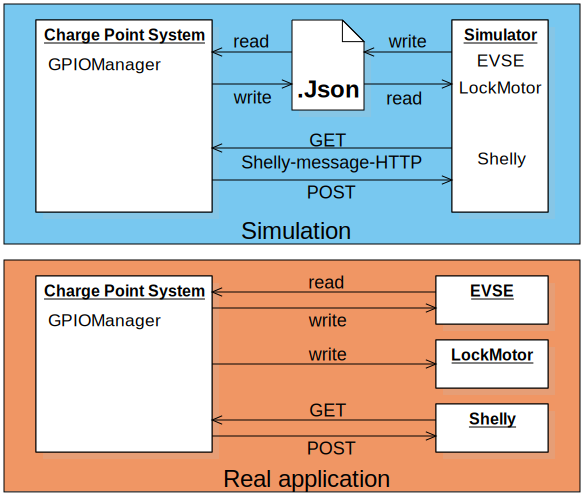
\includegraphics[width=0.66\linewidth]{img/Simulation.png}
            \caption{Simulation VS. reality}
            \label{fig:SimulationFrame}
        \end{figure}


        % \paragraph{模拟器实现}
        % 该模拟器采用PyQt5进行开发,并提供可视化界面,方便用户查看和调整模拟参数。为了便于分发和使用,模拟器最终通过PyInstaller进行打包,以生成独立可执行文件,使其能够在无需额外安装Python环境的情况下直接运行。本项目打包工具采用PyInstaller-GUI(https://github.com/Jf-JIN/Pyinstaller-GUI/releases/tag/v4.0.1), 使用PyInstaller进行打包。

        % 通过此模拟器即可在安全的测试环境下调试和优化系统的充电控制逻辑,确保功能正确性,并减少直接上电测试可能带来的安全隐患。

        \paragraph{Simulator Implementation}
        The simulator is developed using PyQt5 and provides a visual interface, allowing users to view and adjust simulation parameters. To facilitate distribution and usage, the simulator is packaged using PyInstaller to generate a standalone executable file, enabling it to run directly without the need for an additional Python environment. The packaging tool used for this project is PyInstaller-GUI (\href{https://github.com/Jf-JIN/Pyinstaller-GUI/releases/tag/v4.0.1}{Github-Repo}), which leverages PyInstaller for packaging.(\autoref{fig:Simulator})

        This simulator allows for the debugging and optimization of the system's charging control logic in a safe testing environment, ensuring functionality correctness and reducing the safety risks associated with direct live testing.
        \begin{figure}[H]
            \centering
            \includegraphics[width=0.5\linewidth]{img/Simulator.png}
            \caption{GUI of Simulator}
            \label{fig:Simulator}
        \end{figure}


        % \section{充电桩组装与测试}
        \section{Charging Point Assembly and Testing}
        \label{sec:assembleAndTest}
        % 这里还没有写,一方面上次忘了拍图片,下周二咱们记得点拍照。另一方面……不知道写啥 >_<||
        (Because the assembly and testing are not complete yet, so we haven't written this section.)








        % % chapter 9
        % \chapter{Results}
        % 实际所实现的功能(分软硬件),如优化器,充电桩网页数据实时展示以及通过特定csv来自定义充电等等
        % chapter 10
        \chapter{Results \& Discussion}
        % 本章节总结了当前系统在功能设计、技术实现及未来优化方向上的一些关键问题和改进建议。
        % \section{Results}
        % 在本项目中,我们成功实现了以下任务:
        % \begin{enumerate}
            %     \item 充电桩控制与优化\\
            %     充电桩的控制基于充电计划表,该计划表可根据不同的策略进行动态调整,如动态充电、最短时间充电,最少费用充电。使得系统能够选择在最佳时间段内进行充电,降低电网压力。
            %     \item 充电桩与优化器的通讯机制\\
            %     本项目中实现了充电桩与优化器基于OCPP协议的通讯机制,使得充电桩能够与优化器交互,并实现充电任务的智能管理和实时数据更新
            %     \item 简单的数据可视化\\
            %     为了方便查看充电过程,我们实现了简单的数据可视化,包括充电电量曲线,充电计划电量曲线,充电过程中的功率变化曲线,优化前后家庭的用电功率与电网最大功率。
            %     \item GUI 界面设计\\
            %     本项目提供了一个 简洁易用的图形用户界面(GUI),用于显示充电状态、日志信息以及控制操作。该界面支持基本的用户交互,如启动/停止充电、充电模式选择、提交充电计划请求、执行手动上传的充电计划表,远程管理等,方便对充电桩进行监控和控制。
            %     \item 充电过程的软件模拟\\
            %     为了在开发和测试阶段减少对真实硬件的依赖,提高上电测试时的安全,我们实现了充电过程的软件模拟。该模拟系统能够模拟真实的充电流程,包括充电开始、充电中、充电完成等多个阶段,并能够生成相应的状态数据,以便在实验环境下进行调试和优化。
            %     \item 充电桩的改装与优化\\
            %     本项目不仅涉及软件系统的开发,还对充电桩进行了 硬件改装和优化,以提高其兼容性和智能化水平。改装工作包括:
            %     \begin{itemize}
                %         \item 使用EVSE控制充电
                %         \item 增加对充电时电流监控的传感器Shelly
                %         \item 通过RaspberryPi和搭载的脚本控制EVSE和Shelly,实现智能充电
                %     \end{itemize}
            % \end{enumerate}
        \section{Results}
        In this project, we have successfully achieved the following tasks:

        \begin{enumerate}
            \item \textbf{Charging point Control and Optimization}\\
            The control of the charging point is based on a charging schedule, which can be dynamically adjusted according to different strategies, such as dynamic charging, shortest-time charging, and lowest-cost charging. This enables the system to select the optimal charging time slots, reducing the burden on the power grid.

            \item \textbf{Communication Mechanism Between Charging point and Optimizer}\\
            We have implemented a communication mechanism based on the OCPP protocol, allowing the charging point to interact with the optimizer for intelligent charge management and real-time data updates.

            \item \textbf{Simple data visualization}\\
            In order to facilitate the viewing of the charging process, we have realized simple data visualization, including charging capacity curve and charging power plan curve, power change curve during charging, household power consumption and maximum power of the grid before and after optimization.

            \item \textbf{GUI Design}\\
            The project provides a simple and user-friendly Graphical User Interface (GUI) to display charging status, log information, and control operations. This interface supports basic user interactions such as starting/stopping charging, selecting charging modes, submitting charging schedule requests, executing manually uploaded schedules, and remote management, making it easier to monitor and control the charging point.

            \item \textbf{Software Simulation of the Charging Process}\\
            To reduce dependency on real hardware during development and testing, as well as to enhance safety during power-on testing, we implemented a software simulation of the charging process. This simulation system can emulate real charging scenarios, including before charging, in charging, and after charging. It also generates corresponding status data, allowing for debugging and optimization in an experimental environment.

            \item \textbf{Charging point Modification and Optimization}\\
            This project involves not only software system development but also hardware modifications and optimizations of the charging point to improve its compatibility and intelligence. The modifications include:
            \begin{itemize}
                \item Using EVSE for charging control.
                \item Adding a Shelly sensor to monitor charging current.
                \item Control EVSE and Shelly through RaspberryPi with the script to achieve smart charging.
            \end{itemize}
        \end{enumerate}

        \section{Discussion}
        This section summarizes some key issues and improvement suggestions for the current system in terms of functional design, technical implementation and future optimization directions.
        \begin{enumerate}

            % \item 并发消息处理问题\\
            % 目前,系统在 OCPP 消息的并发处理方面存在一定限制。正如 \ref{sec:ocppLib} 所述,官方提供的 OCPP Python 库默认不支持并发处理消息,因此当系统需要同时处理多个 OCPP 请求时,可能会导致阻塞或延迟,影响充电桩的实时控制能力。如果未来系统需要处理高并发 OCPP 消息交互,可以参考 \ref{sec:ocppLib} 中提供的解决方案,对 OCPP 处理逻辑进行优化,以提升消息处理的并发程度。
            \item Concurrent Message Processing Issues\\
            Currently, the system has certain limitations in handling concurrent OCPP messages. As mentioned in \ref{sec:ocppLib}, the official OCPP Python library does not  support concurrent message processing. Consequently, when the system needs to handle multiple OCPP requests simultaneously, it may lead to blocking or delays, affecting the real-time control capability of the charging station. If the system requires high-concurrency OCPP message interactions in the future, the solutions provided in \ref{sec:ocppLib} can be referenced to optimize the OCPP processing logic and enhance message processing concurrency.

            % \item 电流监控与安全控制
            % 当前系统在充电过程中 没有对电流参数进行监控和限制,这可能会导致以下问题:
            %     \begin{itemize}
                %         \item 电流抖动:在某些情况下,电流可能会出现较大的波动,影响充电稳定性。
                %         \item 电流激增:当负载突然增大时,可能会导致电流急剧上升,进而影响供电系统的安全性。
                %     \end{itemize}

            \item Current Monitoring and Safety Control\\
            Currently, the system does not monitor or limit current parameters during the charging process, which may lead to the following issues:
            \begin{itemize}
                \item Current Fluctuations: In certain situations, the current may experience significant variations, affecting charging stability.
                \item Current Surges: A sudden increase in load may cause a sharp rise in current, which potentially affects the safety of the power supply system.
            \end{itemize}

            % 为提升安全性和可靠性,未来可以在Shelly模块中增加电流监控及数据过滤机制
            % 例如:设定电流波动的阈值,若超出范围则进行报警提示,并限制其最大值为阈值。在异常电流激增时,触发保护机制,自动断开充电,防止设备损坏或安全事故发生。
            To enhance safety and reliability, current monitoring and data filtering mechanisms can be added to the Shelly module in the future.
            For example, a threshold for current fluctuations can be set. If the fluctuation exceeds the predefined range, an alarm notification will be triggered, and the maximum current will be limited to the threshold value.
            In the event of an abnormal current surge, a protection mechanism will be activated to automatically stop charging, preventing equipment damage or potential safety incidents.


            % \item 多充电口图像显示支持
            % 目前,网页前端的充电状态图像显示功能,不支持动态增减充电口,即当前UI仅适用于固定数量的充电单元。如果未来需要支持 多个充电单元的动态管理,则需要对前端进行适配
            \item Multi-Charging Port Image Display Support\\
            Currently, the charging status image display function on the web front-end does not support dynamically adding or removing charging ports. The current UI is only applicable to a fixed number of charging units. If future requirements include dynamic management of multiple charging units, the front-end will need to be adapted accordingly.


            % \item EVSE和Shelly的动态注册
            % 目前,EVSE和Shelly的注册是通过枚举类进行的,这种方式的缺点是 新增或移除充电单元需要修改代码并重启系统。为提升灵活性,未来可以改进为基于文件或数据库的动态注册机制。
            \item Dynamic Registration of EVSE and Shelly\\
            Currently, the registration of EVSE and Shelly is implemented through an enumeration class. The drawback of this approach is that adding or removing charging units requires modifying the code and restarting the system. To enhance flexibility, a dynamic registration mechanism based on files or a database can be introduced in the future.


            % \item 网页的终端消息显示限制
            % 目前网页前端没有对消息显示的限制,当系统运行较久且网页长期未刷新,则可能出现内存溢出或浏览器崩溃的问题。为避免该问题,应对显示消息做一定的限制,具体消息通过日志文件进行查看。
            \item Limitation on Web Terminal Message Display\\
            Currently, the web front-end does not impose any limits on message display. If the system runs for a very long period and the webpage is not refreshed for a long time, it may lead to memory overflow or browser crashes. To prevent this issue, a restriction should be applied to the number of displayed messages, while detailed logs can be accessed through log files.


            % \item 树莓派WiFi热点支持
            % 目前,本系统运行在树莓派上,但当前的树莓派 无法开启WiFi热点。这意味着,当树莓派的WiFi连接不稳定或无法连接时,系统管理和远程访问将变得不方便。如果未来的树莓派硬件或系统可以使用WiFi热点功能,则可以考虑在树莓派上启用AP模式,允许用户直接连接到树莓派进行管理。

            \item Raspberry Pi WiFi Hotspot Support\\
            Currently, the system runs on a Raspberry Pi, but the existing Raspberry Pi model cannot set up WiFi hotspot. This means that when the WiFi connection on the Raspberry Pi is unstable or cannot be connected, the system management and remote access become inconvenient. If future Raspberry Pi hardware or the system supports the WiFi hotspot function, enabling AP mode on the Raspberry Pi could be considered, allowing users to connect directly to the Raspberry Pi for management.


            % \item OCPP的Python库的兼容性问题
            % 目前,系统所使用的OCPP的Python库存在兼容性问题,特别是在枚举类方面不兼容。由于官方库的更新较慢,未来若要更好适配哥哥OCPP版本,可能需要自行修改OCPP库代码或完全自定义OCPP库,以满足特定业务需求。
            \item Compatibility Issues with the OCPP Python Library\\
            Currently, the OCPP Python library used in the system has compatibility issues, particularly with the enumeration classes. Due to the slow updates of the official library, in order to better adapt to future versions of OCPP, it may be necessary to modify the OCPP library code or fully customize the OCPP library to meet specific business requirements.


            % \item CSMS功能的扩展
            % 目前,CSMS仅实现了基本的充电管理功能,尚未包含更全面的管理功能,例如:
            %     \begin{itemize}
                %         \item 数据库支持:用于记录历史充电数据,便于后续数据分析和优化。
                %         \item 多充电桩管理:当前系统只适用于单个充电桩的管理,未来如果需要支持多个充电桩,则需要扩展 CSMS 的架构,使其能够管理多个充电桩的状态、功率分配和充电计划。
                %         \item 用户权限控制:增加不同级别的用户管理功能,例如管理员可以修改系统设置,而普通用户只能查看充电状态或提交充电请求。
                %     \end{itemize}
            \item Expansion of CSMS Functions\\
            Currently, the CSMS only implements basic charging management functions and does not include more comprehensive management features, such as:
            \begin{itemize}
                \item \textbf{Database Support:} To record historical charging data for subsequent data analysis and optimization.
                \item \textbf{Multi-Charger Management:} The current system is designed for the management of a single charging point. If future support for multiple charging points is required, the CSMS architecture will need to be expanded to manage the status, power distribution, and charging plans of multiple charging points.
                \item \textbf{User Access Control:} Adding user management features with different levels of access, for example, administrators can modify system settings, while regular users can only view the charging status or submit charging requests.
            \end{itemize}

        \end{enumerate}

        % chapter 11

        \printbibliography

        % chapter 12
        \chapter{Appendices}
        \begin{enumerate}
            \item Ladestation\_v2R
            \item Use Case Diagram
            \item Classes Diagram 1
            \item Classes Diagram 2
            \item Components Diagram
            \item Flow Diagram
            \item Simulation test cases
        \end{enumerate}

        \phantomsection
        \addcontentsline{toc}{section}{Ladestation\_v2R}
        \label{add:Ladestation_v2R}
        \includepdf[pages=-]{Ladestation_v2R.pdf}
        \addcontentsline{toc}{section}{Use Case Diagram}
        \includepdf[pages=-]{UseCaseDiagram.pdf}
        \addcontentsline{toc}{section}{Classes Diagram 1}
        \includepdf[pages=-]{ClassesDiagram1.pdf}
        \addcontentsline{toc}{section}{Classes Diagram 2}
        \includepdf[pages=-]{ClassesDiagram2.pdf}
        \addcontentsline{toc}{section}{Components Diagram}
        \includepdf[pages=-]{ComponentDiagram.pdf}
        \addcontentsline{toc}{section}{Flow Diagram}
        \includepdf[pages=-]{FlowDiagram.pdf}
        \addcontentsline{toc}{section}{Simulation test cases}
        \includepdf[pages=-]{TestCases.pdf}

    \end{document}
